% !TEX TS-program = pdflatexmk

% ###################################################################
% Copyright (c) 2017-2018, Editors: A.D. Rollett & M. De Graef
% All rights reserved.
%
% Licensed under the Creative Commons CC BY-NC-SA 4.0 License, 
% hereafter referred to as the "License"; you may not use this 
% document except in compliance with the License. You may obtain 
% a copy of the License at 
%     https://creativecommons.org/licenses/by-nc-sa/4.0/legalcode
% Unless required by applicable law or agreed to in writing, all 
% material distributed under the License is distributed on an 
% "AS IS" BASIS, WITHOUT WARRANTIES OR CONDITIONS OF ANY KIND, 
% either express or implied. See the License for the specific 
% language governing permissions and limitations under the License.
% ###################################################################

\documentclass[11pt,fleqn,A4paper]{book} % Default font size and left-justified equations

% load the OpenChapters.sty package file that loads everything else...
\usepackage{OpenChapters}

% uncomment the chapter you wish to typeset from the list below; to typeset the
% entire text, leave all lines commented
%\includeonly{src/Crystallography/Crystallography}
%\includeonly{src/Symmetry/Symmetry}
%\includeonly{src/2Drotations/2Drotations}
%\includeonly{src/3Drotations/3Drotations}
%\includeonly{src/RotationSymmetry/RotationSymmetry}
%\includeonly{src/Misorientations/Misorientations}
%\includeonly{src/MaterialProperty/MaterialProperty}
%\includeonly{src/PropertyTensors/PropertyTensors}
%\includeonly{src/PropertySymmetry/PropertySymmetry}
%\includeonly{src/ExampleProperties/ExampleProperties}


\begin{document}

% !TEX root = ../Build/main.tex
% ###################################################################
% Copyright (c) 2017-2018, Editors: A.D. Rollett & M. De Graef
% All rights reserved.
%
% Licensed under the Creative Commons CC BY-NC-SA 4.0 License, 
% hereafter referred to as the "License"; you may not use this 
% document except in compliance with the License. You may obtain 
% a copy of the License at https://creativecommons.org/licenses/by-nc-sa/4.0/legalcode. 
% Unless required by applicable law or agreed to in writing, all 
% material distributed under the License is distributed on an 
% ``AS IS'' BASIS, WITHOUT WARRANTIES OR CONDITIONS OF ANY KIND, 
% either express or implied. See the License for the specific language 
% governing permissions and limitations under the License.
% ###################################################################

%----------------------------------------------------------------------------------------
%	TITLE PAGE
%----------------------------------------------------------------------------------------

\renewcommand{\chaptergraphicspath}{matter/eps/}

\begingroup
\thispagestyle{empty}
\begin{tikzpicture}[remember picture,overlay]
\coordinate [below=12cm] (midpoint) at (current page.north);
\node at (current page.north west)
{\begin{tikzpicture}[remember picture,overlay]
\node[anchor=north west,inner sep=0pt] at (0,0) {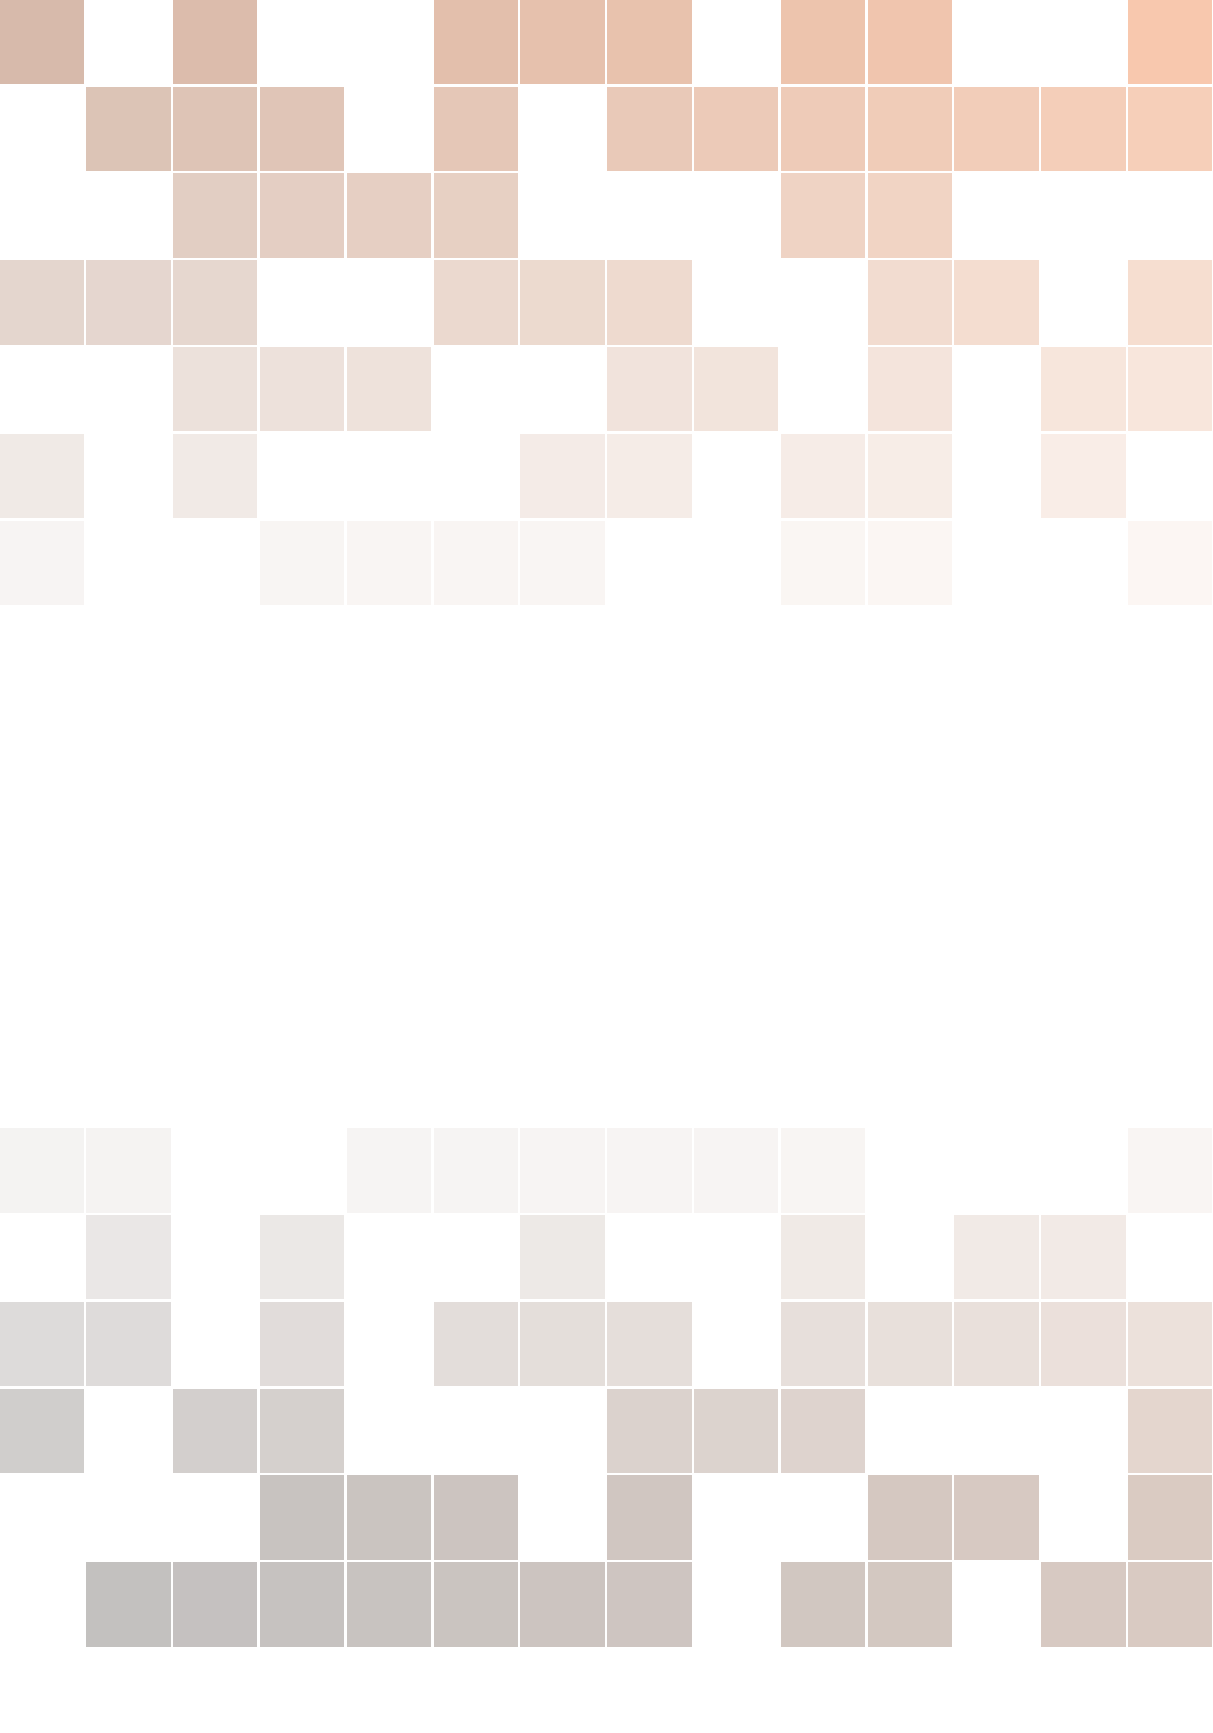
\includegraphics[width=\paperwidth]{background}}; % Background image
% the book title may become a user defined variable in a later version
\draw[anchor=north] (midpoint) node [fill=ocre!30!white,fill opacity=0.6,text opacity=1,inner sep=1cm]{\Huge\centering\bfseries\sffamily\parbox[c][][t]{\paperwidth}{\centering 3D Microstructure and Properties\\ of Crystalline Materials\\[15pt] % Book title
% book subtitle
{\Large A Guide for Materials Scientists and Engineers, Physicists, and Geologists}\\[20pt] % Subtitle
% Author name(s) should go here
% and editor names here
{\huge Anthony D. Rollett and Marc De Graef}}};
\end{tikzpicture}};
\end{tikzpicture}
\vfill
\endgroup

%----------------------------------------------------------------------------------------
%	COPYRIGHT PAGE
%----------------------------------------------------------------------------------------

\newpage
~\vfill
\thispagestyle{empty}

\noindent Copyright \copyright\ 2017-2018 Editors: Anthony D. Rollett and Marc De Graef\\ % Copyright notice

\noindent \textsc{Published by OpenChapters}\\ % Publisher

\noindent \textsc{OpenChapters.web.cmu.edu}\\ % URL

\noindent Licensed under the Creative Commons CC BY-NC-SA 4.0 License, hereafter referred to as the ``License''); you may not
use this document except in compliance with the License. You may obtain a copy
of the License at \url{https://creativecommons.org/licenses/by-nc-sa/4.0/legalcode}. Unless
required by applicable law or agreed to in writing, all material distributed
under the License is distributed on an ``AS IS'' BASIS, WITHOUT
WARRANTIES OR CONDITIONS OF ANY KIND, either express or implied. See the
License for the specific language governing permissions and limitations
under the License.\index{license}\\ % License information

\noindent \textit{First printing, \monthyear} % Printing/edition date

%----------------------------------------------------------------------------------------
%	TABLE OF CONTENTS
%----------------------------------------------------------------------------------------

\chapterimage{chapter_head_1.pdf} % Table of contents heading image
\pagestyle{empty} % No headers
\tableofcontents % Print the table of contents itself
\cleardoublepage % Forces the first chapter to start on an odd page so it's on the right
\pagestyle{fancy} % Print headers again

% not sure if we need this in the front or back matter...
%%\listoffigures
%
%%\listoftables
%
%% dedication
%\cleardoublepage
%~\vfill
%\begin{doublespace}
%\noindent\fontsize{18}{22}\selectfont\itshape
%\nohyphenation
%Dedicated to $\ldots$.
%\end{doublespace}
%\vfill
%\vfill



\cleardoublepage
\chapterimage{chapter_head_2.pdf} % Chapter heading image

\chapter*{Preface}

% the following sections should really come from user-defined text (except for the last one) since this
% will be different for each custom text book...
 
\section*{Who should read this book?}



\section*{What is in this book?}
We begin this book with rotations in 2D; this will serve as a review as well as an opportunity to define several important concepts, including \textit{active} and \textit{passive} rotations, \textit{positive} and \textit{negative} rotation angles, and so on.  Then we cover 3D rotations in section~\ref{sec:3Drotations} using only rotation matrices; we will introduce the concept of a special orthonormal matrix and the related space of 3D orientations, $SO(3)$.  Euler angles form the topic of section~\ref{sec:eulerangles}; we will introduce the Bunge convention in detail, and also discuss other conventions.  Neo-Eulerian representations are introduced in section~\ref{sec:neoEulerian}; they include the \textit{axis-angle pair}, the \textit{quaternion}, the \textit{Rodrigues-Frank vector}, the \textit{homochoric vector}, and the \textit{stereographic vector}.  Section~\ref{sec:cubochoric} is devoted to the recently introduced \textit{cubochoric} representation.



The text is heavily illustrated and makes use of numerous examples and exercises.  





\section*{What does Open Source mean for this book?}
This is an \textit{open source}\index{open source} book, meaning that, in addition to this PDF file, we make all the original \LaTeX\ source files and original illustrations available on-line via the GitHub repository.  The copyright for this book falls under the \textit{Creative Commons Attribution-NonCommercial-ShareAlike 4.0 International Public License}\index{license} or CC BY-NC-SA 4.0 for short.  If you are just a reader interested in the material covered in this book, then you do not need to think about this copyright license at all.  If you are a researcher who wishes to use some of the illustrations for your own publications, or if you are an instructor who would like to make printed copies of this text available to a group of students, or if you wish to contribute to this text, then we encourage you to read the detailed license available from \url{https://creativecommons.org/licenses/by-nc-sa/4.0/legalcode}. 

Here is what it means in practice (text taken from the Creative Commons web site): 
{\small\begin{itemize}
	\item \textit{\textbf{Sharing:}} you are free to copy and redistribute this material in any medium or format;
	\item \textit{\textbf{Adapting:}} you are free to remix, transform, and build upon this material. 
\end{itemize}}
\noindent You have these freedoms as long as you follow the license terms:
{\small\begin{itemize}
	\item \textit{\textbf{Attribution:}}  you must give appropriate credit, provide a link to the license, and indicate if changes were made. You may do so in any reasonable manner, but not in any way that suggests the licensor endorses you or your use;
	\item \textit{\textbf{NonCommercial:}} you may not use the material for any commercial purposes;
	\item \textit{\textbf{ShareAlike:}} if you remix, transform, or build upon the material, you must distribute your contributions under the same license as the original.
\end{itemize}}
You may not apply legal terms or technological measures that legally restrict others from doing anything the license permits.







% Here are all the parts and chapters

% ###################################################################
\part{Foundations}
% ###################################################################
% !TEX root = ../../Build/main.tex
% ###################################################################
% Copyright (c) 2018, Marc De Graef 
%  Editors: A.D. Rollett & M. De Graef
% All rights reserved.
%
% Licensed under the Creative Commons CC BY-NC-SA 4.0 License, 
% hereafter referred to as the "License"; you may not use this 
% document except in compliance with the License. You may obtain 
% a copy of the License at 
%     https://creativecommons.org/licenses/by-nc-sa/4.0/legalcode 
% Unless required by applicable law or agreed to in writing, all 
% material distributed under the License is distributed on an 
% "AS IS" BASIS, WITHOUT WARRANTIES OR CONDITIONS OF ANY KIND, 
% either express or implied. See the License for the specific 
% language governing permissions and limitations under the License.
% ###################################################################

% ###################################################################
% The following lines are to be uncommented or edited as needed 

\corechapter{Yes}
%     uncomment this line only if this chapter is a core/foundational chapter;
%     for a core chapter a "Core" label will appear on the top left above the chapter title.

\chapterauthor{Marc De Graef, Carnegie Mellon University}
%     this will appear in a secondary header below the chapter title.

% All figures are stored in the src/Crystallography/eps folder and must be of the *.eps type. 
\renewcommand{\chaptergraphicspath}{src/Crystallography/eps/}

\chapterimage{\noheaderimage}
%     replace \noheaderimage by the chapter header image file name (without .eps extension).
%     Chapter header images must be 2480 x 1240 pixels with 300dpi, RGB format.
% ###################################################################

\chapter{Basic Crystallography\label{chap:Crystallography}}



\section{Notational Conventions in Cartesian Reference Frames\label{ssec:notations}}
We will represent vectors by bold symbols, e.g.,  $\mathbf{a}$, $\mathbf{b}$, $\ldots$.  Unless stated otherwise, we will work with Cartesian (i.e., orthonormal) reference frames\index{Cartesian reference frame}; Cartesian basis vectors\index{Cartesian basis vector} will always be represented by vectors of the type $\mathbf{e}_i$, where the subscript $i$ can take on the values $1, 2, \ldots, D$ and $D$ is the dimension of the space in which the vectors live.  Occasionally, the subscript $i$ will be interpreted to mean $x, y$ in 2D and $x,y,z$ in 3D; this will be clear from the context, and usually this notation is only used to clarify things.  Note that vectors represented by the letter ``\textbf{e}'' will always be assumed to be unit vectors.\index{unit vector}

\begin{wrapfigure}{r}{0.3\textwidth}
  \centering\leavevmode
\Ovalbox{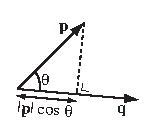
\includegraphics[width=0.28\textwidth]{dotproduct}}
\caption{\small Illustration of the vector dot product as the projection of $\mathbf{p}$ onto $\mathbf{q}$, multiplied by the length $\vert\mathbf{q}\vert$.\label{fig:dp}}
\end{wrapfigure}

The dot product\index{dot product} between two vectors (see Fig.~\ref{fig:dp}) is denoted by the symbol $\cdot$, as in:
\begin{equation}
	\mathbf{p}\cdot\mathbf{q} = \vert\mathbf{p}\vert\vert\mathbf{q}\vert\cos\theta \ ,\label{eq:dotproduct}
\end{equation}
where $\vert\mathbf{p}\vert$ stands for the norm (length) of the vector $\mathbf{p}$, and $\theta$ is the angle between the two vectors. When two vectors are perpendicular to each other, then their dot product vanishes.  The dot product of a vector with itself results in the square of the length of the vector, or
\begin{equation}
	\vert\mathbf{p}\vert = \sqrt{\mathbf{p}\cdot\mathbf{p}} \ .\label{eq:vectorlength}
\end{equation}

The vector cross product\index{vector cross product}\index{cross product} is represented by the symbol $\times$, as in
\begin{equation}
	\mathbf{p}\times\mathbf{q} = \vert\mathbf{p}\vert\vert\mathbf{q}\vert \sin\theta\ \mathbf{e}^{\perp} \ ,\label{eq:crossproduct}
\end{equation}
Here, the unit vector $\mathbf{e}^{\perp}$ is perpendicular to both $\mathbf{p}$ and $\mathbf{q}$, such that $\mathbf{p}$, $\mathbf{q}$ and $\mathbf{e}^{\perp}$ form a right-handed reference frame.\footnote{In crystallography and texture analysis we always use right-handed reference frames. Left-handed frames are common in computer vision and animation.}   The cross product of a vector with itself always vanishes. The mixed vector product,\index{mixed vector product} $\mathbf{p}\cdot(\mathbf{q}\times\mathbf{r})$, is equal to the volume, $V$, of the parallellepiped generated by the three vectors.  For a right-handed reference frame, the mixed vector product is always positive; for  a left-handed reference frame it is negative.

Vector components are represented by subscripted italic symbols; the Cartesian components of the vector $\mathbf{p}$ can be determined by projecting the vector onto each coordinate axis using the dot product.  Thus, we have:
\begin{equation}
	\mathbf{p} = \sum_{i=1}^{D}(\mathbf{p}\cdot\mathbf{e}_i)\mathbf{e}_i = \sum_{i=1}^D p_i\mathbf{e}_i \ .
\end{equation}
We will use the Einstein summation convention:\index{summation convention} \textit{when a subscript is present twice on the right hand side of an equation, a summation over that subscript is implied and the summation sign need not be written}.  
Thus, we have:
\begin{equation}
	\mathbf{p} = p_i\mathbf{e}_i\quad\text{with}\quad p_i = \mathbf{p}\cdot\mathbf{e}_i \ .
\end{equation}

\noindent In component notation, the vector dot and cross products can be written explicitly as follows:
\begin{itemize}
	\item For the dot product between $\mathbf{p}$ and $\mathbf{q}$ we have:
	\[
		\mathbf{p}\cdot\mathbf{q} = (p_i\mathbf{e}_i)\cdot(q_j\mathbf{e}_j)
		= p_i (\mathbf{e}_i\cdot\mathbf{e}_j) q_j \ .
	\]
	The dot product of the orthonormal basis vectors is equal to $1$ for $i=j$ or $0$ for $i\ne j$; we represent this by the Kronecker symbol\index{Kronecker symbol} $\delta_{ij}$, which corresponds to the $D$-dimensional identity matrix:
	\[
		\mathbf{p}\cdot\mathbf{q} = p_i \delta_{ij} q_j \ .
	\]
	Carrying out the summation over $j$ we obtain:
	\[
		\mathbf{p}\cdot\mathbf{q} = p_i q_i \quad [=p_1q_1+p_2q_2+\ldots ]\ .
	\]
	Using $x,y,\ldots$ as the subscripts, we obtain the familiar expression $\mathbf{p}\cdot\mathbf{q} =p_xq_x+p_yq_y+\ldots$.
	\item For the vector cross product we have:
	\[
		\mathbf{p}\times\mathbf{q} = p_iq_j \epsilon_{ijk} \mathbf{e}_k \ ,
	\]
	where $\epsilon_{ijk}$ is the permutation symbol\index{permutation symbol}; this symbol is equal to $+1$ if $ijk$ is an even permutation of $123$, $-1$ for an odd permutation, and $0$ whenever two or more of the indices are equal.  This definition leads to the familiar expression:
	\[
		\mathbf{p}\times\mathbf{q} = (p_2q_3-p_3q_2)\mathbf{e}_1 +(p_3q_1-p_1q_3)\mathbf{e}_2 +(p_1q_2-p_2q_1)\mathbf{e}_3 \ .
	\] 
\end{itemize}

\section{Real Space and Reciprocal Space\label{ssec:spaces}}
After teaching crystallography for several decades as well as writing an extensive textbook on the topic, it has become clear to the author that many students and researchers tend to have an incomplete and sometimes incorrect understanding of the reasons for using both real and reciprocal space.  So, before we introduce these important crystallographic concepts, it is important to ensure that the reader understand why these two spaces are necessary and, more importantly, that they represent two natural ways to look at and describe crystal structures.  There is nothing difficult or mysterious about reciprocal space, in particular.

Let us begin with a familiar example.  A street is lined with a series of trees, planted at a regular distance from each other;  Fig.~\ref{fig:trees} shows a schematic of a portion of this street.  We take a measuring stick of a given length $S$, and measure the distance $d$ between two consecutive trees in units of $S$.  For the illustration in Fig.~\ref{fig:trees}(a) we find that $d=1$ S.  Next, we double the length of the measuring stick to $S'=2S$ and once again we measure the distance $d$; this time we find $d = 1/2$ S'.  Now we make the following, almost trivial, observation: \textit{when the length of the measuring stick increases, the numerical value of the distance decreases.} In other words, the length of the measuring stick and the measured quantity vary in opposite ways; when one becomes larger, the other becomes smaller and vice versa.  Hence, we say that the distance between the trees is a \textit{contravariant}\index{contravariant} quantity (``contra'' means ``opposite'' in this context); it varies in the opposite way from the units in which it is measured.

\begin{wrapfigure}{r}{0.3\textwidth}
  \centering\leavevmode
%\Ovalbox{\includegraphics[width=0.28\textwidth]{trees}}
\caption{\small Illustration of the measurement of (a) the distance between trees (a contravariant quantity) and (b) the number of trees per unit distance (a covariant quantity).\label{fig:trees}}
\end{wrapfigure}

Next, we rephrase the question about the distance between trees as follows: \textit{how many trees are there per unit distance $T$?}  From Fig.~\ref{fig:trees}(b) we find that there are $r=2$ trees per unit distance $T$, or $r=2$ T$^{-1}$.  Doubling the measuring stick to $T'=2T$, we find that $r=4$ T'$^{-1}$.  Interestingly, in this case both the measuring unit and the quantity measured vary in the same way; when one becomes larger, so does the other.  Therefore, the number of trees per unit length is a \textit{covariant}\index{covariant} quantity (``co'' meaning ``with'' or ``in the same way''); it varies in the same way as the units in which it is measured.

Clearly, the row of trees is the same in both cases, but we simply consider the separation between the trees in two different ways: ``distance between trees'' and ``number of trees per unit distance.''  Replacing trees by planes of atoms, the first approach yields direct or real space, the second yields reciprocal space.\footnote{It is possible to generalize the subscript notation introduced above to one that uses both subscripts and superscripts; this is standard in some branches of physics and leads to an explicit distinction between contravariant and covariant vector components. While it is possible to rewrite this entire book using covariant and contravariant notations, we opt not to do so and we will use only subscripts to indicate vector (and tensor) components.}  It is that simple!   In the direct space description of crystal structures we think about the distances between atoms or crystal planes in terms of contravariant quantities (the actual distances in units of length); in the reciprocal space description we think instead about the number of lattice planes per unit distance, i.e., in terms of covariant quantities (number of planes per unit length, or lineal density).  Since both quantities $d$ and $r$ in the tree example describe \textit{the same row of trees}, direct and reciprocal space describe \textit{the same crystal structure}; we simply use different units for each description.  

So, if the distinction between direct and reciprocal space is this simple, why is it that so many students and researchers struggle with the concept of reciprocal space? One reason might be the strongly visual way in which our brain works; if you take a model crystal structure in your hands, you can easily visualize the atom locations and distances between the atoms. Hence, direct space is a natural way to describe the crystal structure.  It is a bit more difficult to ``visualize'' the number of atoms per unit length.  Another reason may lie in the choice of words: direct \textit{space} and reciprocal \textit{space}.  This choice seems to imply that somehow there are two different spaces, and that, perhaps, these spaces are in different locations.  This incorrect interpretation is likely due to a misunderstanding of the word \textit{space} in this context; the word should be interpreted as an abbreviation for \textit{vector space}, i.e., a mathematical space created by linear combinations of a set of basis vectors.  Direct and reciprocal space then simply refer to the fact that there are two different sets of basis vectors, i.e., two different sets of measuring sticks, used to generate the vector spaces. So, when we say \textit{direct space}, we really mean \textit{the vector space spanned by the direct basis vectors}, and by \textit{reciprocal space} we mean \textit{the vector space spanned by the reciprocal basis vectors}. Both vector spaces are mapped onto the actual crystal structure, so both vector spaces ``occupy'' the same physical space. Next, we will cast these concepts into more precise mathematical statements.


\section{Crystallographic Conventions and Computations\label{ssec:crystalconventions}}

\subsection{Direct space}
All crystallographic conventions in this book follow the International Tables for Crystallography, Volume A.  In particular, we represent the unit cell\index{unit cell} of a crystal structure\index{crystal structure} by means of the basis vector\index{basis vectors!crystallographic} triplet $\{\mathbf{a}_i\}$ with $i=1,\ldots,3$ or $\{\mathbf{a}, \mathbf{b},\mathbf{c}\}$ (see Fig.~\ref{fig:unitcell}). The subscripted notation for the basis vectors is much more convenient for analytical calculations, so we will use it whenever possible. The lattice parameters\index{lattice parameters} of the unit cell are the six numbers $\{a,b,c,\alpha,\beta,\gamma\}$, where $a, b, c$ are the lengths of the vectors $\mathbf{a}_1$, $\mathbf{a}_2$, and $\mathbf{a}_3$, respectively, and $\alpha=\text{ang}(\mathbf{a}_2,\mathbf{a}_3)$,  $\beta=\text{ang}(\mathbf{a}_1,\mathbf{a}_3)$,  and $\gamma=\text{ang}(\mathbf{a}_1,\mathbf{a}_2)$, where $\text{ang}(\mathbf{p},\mathbf{q})$ stands for the angle between the vectors $\mathbf{p}$ and $\mathbf{q}$.

\begin{wrapfigure}{r}{0.3\textwidth}
  \centering\leavevmode
%\Ovalbox{\includegraphics[width=0.28\textwidth]{unitcell}}
\caption{\small Illustration of the basis vectors of a crystallographic unit cell.\label{fig:unitcell}}
\end{wrapfigure}

The crystallographic basis vectors can be used to generate a vector space\index{vector space} by considering all linear combinations of the three vectors. Among these linear combinations, integer linear combinations are of special importance since they correspond to the translation vectors that allow one to jump from the corner of any one unit cell to that of any other unit cell.  For an integer triplet $(u,v,w)$, or $u_i\in\mathbb{Z}$ in component form, we define the lattice translation vector\index{lattice translation vector} $\mathbf{t}_{uvw}$ as
\begin{equation}
	\mathbf{t}_{uvw} = u_i\mathbf{a}_i = u\mathbf{a}_1+v\mathbf{a}_2+w\mathbf{a}_3 \ .
\end{equation}
The integer triplet is often written as $[uvw]$ and represents a direction in the crystal lattice; this notation is valid for all crystal systems. So, the direction triplet $[120]$ represents the lattice translation vector $\mathbf{t}=\mathbf{a}_1+2\mathbf{a}_2$ in \textit{any} crystal system. Negative components are denoted by putting the minus sign above the corresponding digit, as in $[1\bar{1}2]$. Atom positions inside the unit cell are represented by fractional position vectors $\mathbf{r}_j$ with components $r_{j,i}=(x_j,y_j,z_j)\in [0,1]$; the subscript $j$ indicates the atom label in case there is more than one atom in the cell.  The subscript $i$ labels the components of the position vector. The numbers $r_{j,i}$ are known as the fractional coordinates\index{fractional coordinates} of atom $j$.

\subsection{Direct Space Computations} 
We can use the dot product defined in a previous section to derive expressions for the distance between points, and the angle between direction vectors. Consider an atom at position $\mathbf{r}$ in an arbitrary unit cell; the length of the vector $\mathbf{r}$ is given by equation~\ref{eq:vectorlength}:
\[
	\vert\mathbf{r}\vert = \sqrt{\mathbf{r}\cdot\mathbf{r}} \ .
\]
Substituting the component representation we find:
\begin{align}
	\vert\mathbf{r}\vert^2 &= (r_i\mathbf{a}_i)\cdot(r_j\mathbf{a}_j)\ ;\nonumber\\
	&= r_i (\mathbf{a}_i\cdot\mathbf{a}_j) r_j\ ;\nonumber\\
	&= r_i g_{ij} r_j\ .\label{eq:vectorlength}
\end{align}
We have introduced the symbol $g_{ij}$, defined as:
\begin{equation}
	g_{ij} \equiv \mathbf{a}_i\cdot\mathbf{a}_j \ ;\label{eq:gdirectdef}
\end{equation}
the $3\times 3$ matrix $g_{ij}$ contains the dot products between pairs of basis vectors and is known as the \textit{direct metric tensor}\index{metric tensor!direct} because it defines how distances (and angles) are computed in a non-Cartesian reference frame, i.e., it defines the \textit{metric properties} of the reference frame.

The metric tensor is written explicitly as:
\[
	g_{ij} = \left(\begin{array}{ccc}
	\mathbf{a}_1\cdot\mathbf{a}_1 & \mathbf{a}_1\cdot\mathbf{a}_2 & \mathbf{a}_1\cdot\mathbf{a}_3 \\
	\mathbf{a}_2\cdot\mathbf{a}_1 & \mathbf{a}_2\cdot\mathbf{a}_2 & \mathbf{a}_2\cdot\mathbf{a}_3 \\
	\mathbf{a}_3\cdot\mathbf{a}_1 & \mathbf{a}_3\cdot\mathbf{a}_2 & \mathbf{a}_3\cdot\mathbf{a}_3 \end{array}\right)
	 = \left(\begin{array}{ccc}
	 a^2 & a b \cos\gamma & a c \cos\beta\\
	 a b cos\gamma & b^2 & b c \cos\alpha\\
	 a c \cos\beta & b c \cos\alpha & c^2 \end{array}\right)\ .
\]
In order for the expression in Eq.~\ref{eq:vectorlength} to make mathematical sense in terms of the standard matrix multiplication rules, the components $r_i$ must be written as a $1\times 3$ row vector, whereas the components $r_j$ correspond to the $3\times 1$ column vector.  Thus, the expression reads:
\[
	\vert\mathbf{r}\vert^2 = \left(\begin{array}{ccc}r_1 & r_2 & r_3\end{array}\right)
	 \left(\begin{array}{ccc}
	\mathbf{a}_1\cdot\mathbf{a}_1 & \mathbf{a}_1\cdot\mathbf{a}_2 & \mathbf{a}_1\cdot\mathbf{a}_3 \\
	\mathbf{a}_2\cdot\mathbf{a}_1 & \mathbf{a}_2\cdot\mathbf{a}_2 & \mathbf{a}_2\cdot\mathbf{a}_3 \\
	\mathbf{a}_3\cdot\mathbf{a}_1 & \mathbf{a}_3\cdot\mathbf{a}_2 & \mathbf{a}_3\cdot\mathbf{a}_3 \end{array}\right) 
	\left(\begin{array}{c}r_1\\
	r_2\\
	r_3\end{array}\right)\ .
\]

\begin{example} 
Consider a tetragonal unit cell with lattice parameters $a=2$ and $c=4$ (the units are not important so we omit them here).  All three angles are $90^{\circ}$ so the off-diagonal dot products in the metric tensor vanish, leaving
\[
	g_{ij} = \left(\begin{array}{ccc}
			4 & 0 & 0\\
			0 & 4 & 0\\
			0 & 0 & 16\end{array}\right) \ .
\]
The distance from the origin to an atom at fractional position $\mathbf{r}=(\frac{1}{4},\frac{1}{4},\frac{3}{4})$ is given by:\begin{align*}
	\vert\mathbf{r}\vert^2 &= \left(\begin{array}{ccc}\frac{1}{4} & \frac{1}{4} & \frac{3}{4}\end{array}\right)
			\left(\begin{array}{ccc}
			4 & 0 & 0\\
			0 & 4 & 0\\
			0 & 0 & 16\end{array}\right)
			\left(\begin{array}{c}\frac{1}{4} \\ \frac{1}{4} \\ \frac{3}{4}\end{array}\right)\ ; \\
			&=  \left(\begin{array}{ccc}\frac{1}{4} & \frac{1}{4} & \frac{3}{4}\end{array}\right)
			\left(\begin{array}{c}1 \\ 1 \\ 12\end{array}\right)\ ; \\
			&= \frac{19}{2}\ .
\end{align*}
Thus, we have $\vert\mathbf{r}\vert = \sqrt{19/2} = 3.0822$.
\end{example}

\begin{exercise}
For a monoclinic lattice with lattice parameters $(a,b,c) = (1, 4, 2)$ and $\beta=60^{\circ}$, what is the distance between atoms at fractional positions $(1/2,0,1/2)$ and $(0,1/2,1/2)$?\label{ex:mono}
\end{exercise}

Next, we consider the angle between two directions $\mathbf{s}$ and $\mathbf{t}$.  From the dot product definition we find that
\begin{equation}
	\theta = \text{ang}(\mathbf{s},\mathbf{t}) = \arccos\left( \frac{\mathbf{s}\cdot\mathbf{t}}{\vert\mathbf{s}\vert\vert\mathbf{t}\vert}\right) = 
	\arccos\left( \frac{\mathbf{s}\cdot\mathbf{t}}{\sqrt{\mathbf{s}\cdot\mathbf{s}}\sqrt{\mathbf{t}\cdot\mathbf{t}}}\right) \ .\label{eq:defangle}
\end{equation}
Formally, we can write the two vectors in matrix form and work out the dot product:
\[
	\left(\begin{array}{c}\mathbf{s}\\ \mathbf{t}\end{array}\right)\cdot\left(\begin{array}{cc}\mathbf{s}&\mathbf{t}\end{array}\right)
	 = \left(\begin{array}{cc}\mathbf{s}\cdot\mathbf{s}&\mathbf{s}\cdot\mathbf{t}\\
	\mathbf{t}\cdot\mathbf{s}&\mathbf{t}\cdot\mathbf{t}\end{array}\right) \ .
\]
Note that the $2\times 2$ matrix on the right hand side contains the three dot products that we need to compute the angle.  

\begin{example}
Hence, for the tetragonal structure introduced above, the angle between the vectors $\mathbf{s}=[110]$ and $\mathbf{t}=[011]$ is computed as follows:
\begin{align*}
	\left(\begin{array}{cc}\mathbf{s}\cdot\mathbf{s}&\mathbf{s}\cdot\mathbf{t}\\
	\mathbf{t}\cdot\mathbf{s}&\mathbf{t}\cdot\mathbf{t}\end{array}\right) &= \left(\begin{array}{ccc}1 & 1 & 0\\ 0 & 1 & 1\end{array}\right)
	\left(\begin{array}{ccc}
			4 & 0 & 0\\
			0 & 4 & 0\\
			0 & 0 & 16\end{array}\right)\left(\begin{array}{cc} 1 & 0\\ 1 & 1\\ 0 & 1\end{array}\right)\ ;\\
	&= \left(\begin{array}{ccc}1 & 1 & 0\\ 0 & 1 & 1\end{array}\right)
	\left(\begin{array}{cc} 4 & 0\\ 4 & 4\\ 0 & 16\end{array}\right)\ ; \\
	&= \left(\begin{array}{cc}8 & 4 \\ 4 & 20 \end{array}\right)\ .
\end{align*}
Therefore we have:
\[
	\text{ang}([110],[011]) = \arccos\left(\frac{4}{\sqrt{8}\sqrt{20}}\right) = \arccos\left(\frac{1}{\sqrt{10}}\right) = 71.56^{\circ}\ .
\]
\end{example}

\begin{exercise}
For the unit cell of Exercise~\ref{ex:mono}, compute the angle between the $[111]$ and $[120]$ directions.
\end{exercise}

\subsection{Reciprocal Space}
In this section, we change our viewpoint of a crystal structure from the direct view (involving distances between atoms) to the reciprocal view (involving the number of atoms per unit length).  This means that we change the measuring sticks used to determine crystallographic quantities; a new set of measuring sticks is equivalent to a new set of basis vectors which we denote by $\mathbf{a}^{\ast}_i$.\footnote{In the covariant-contravariant notation, the reciprocal basis vectors would be written as $\mathbf{a}^i$, i.e., with a superscript instead of a subscript.}  The corresponding reciprocal lattice parameters\index{reciprocal lattice parameters} are written as $\{a^{\ast},b^{\ast},c^{\ast},\alpha^{\ast},\beta^{\ast},\gamma^{\ast}\}$.

Since we will discuss the density of atomic planes, we need to have a simple way to label individual sets of lattice planes.  It was realized a long time ago that the facets of natural crystals could be labeled by integer numbers; this is known as the \textit{Law of Rational Indices}.  The intercepts of a facet plane with the three coordinate axes, measured in appropriate units along those axes, are always rational numbers; hence, we can write them as fractions which we can reduce to integers.  Since some planes are parallel to the coordinate axes, they intersect those axes at infinity, so it is more convenient to invert the intercept ratios before converting them to integers.  The resulting integers are typically written as $(hkl)$ and are known as \textit{Miller indices}\index{Miller indices}.  A simple illustration of the process of determining Miller indices is shown in Fig.~\ref{fig:millerindices}.

Measuring the lineal density of atomic planes requires that we specify the direction along which we measure the density; the only logical direction is the one normal to a given set of planes.\footnote{Note that the units of inverse length are also the units of the spatial gradient operator, $\nabla$, which has components $\partial/\partial x_i$.  The gradient operator evokes the notion of \textit{normal}, which is another reason for measuring the lineal density along the normal to the lattice planes, since this is the direction of the maximum density.} The units of lineal density are \textit{per unit length}, usually expressed in nm$^{-1}$.  Traditionally, we use the symbol $\mathbf{g}_{hkl}$ for the lineal density of planes, and we use the Miller indices of the plane as the subscripts to identify a particular set of planes, e.g., $\mathbf{g}_{200}$.

Since we want to measure the lineal density along plane normals, we will define the reciprocal basis vectors in such a way that their integer linear combinations are indeed normal to the lattice planes; and we want those integer triplets to be equal to the plane's Miller indices.  We can accomplish this by defining the reciprocal basis vectors to be normal to the planes formed by pairs of direct basis vectors $\mathbf{a}_i$.  So, we want $\mathbf{a}^{\ast}_1$ to be perpendicular to both $\mathbf{a}_2$ and $\mathbf{a}_3$, i.e., perpendicular to the plane that contains both vectors; it is easy to see that this is the $(100)$ plane.  Using the same process for the other two reciprocal basis vectors we obtain the following relations (using a constant scaling factor $C$):
\begin{align*}
	\mathbf{a}^{\ast}_1 &= C \mathbf{a}_2\times\mathbf{a}_3 \ ;\\
	\mathbf{a}^{\ast}_2 &= C \mathbf{a}_3\times\mathbf{a}_1 \ ;\\
	\mathbf{a}^{\ast}_3 &= C \mathbf{a}_1\times\mathbf{a}_2 \ .	
\end{align*}
To determine the constant $C$, we require that the dot product of $\mathbf{a}_i^{\ast}$ with the corresponding direct basis vector $\mathbf{a}_i$ be equal to $1$; after all, we want the two spaces to be reciprocal to each other.\footnote{Note that, in the physics literature, it is common to insert a factor of $2\pi$ in the definition of $C$, i.e., $C=2\pi/V$.  In the crystallographic community, this factor is usually not included.} Recognizing that the mixed product of the three direct space vectors is the unit cell volume, $V$, we find that $C=1/V=1/\mathbf{a}_1\cdot(\mathbf{a}_2\times\mathbf{a}_3)$.  Hence, the reciprocal basis vectors are defined as:
\begin{align}
	\mathbf{a}^{\ast}_1 &= \frac{\mathbf{a}_2\times\mathbf{a}_3}{V} \ ;\nonumber\\
	\mathbf{a}^{\ast}_2 &= \frac{\mathbf{a}_3\times\mathbf{a}_1}{V} \ ;\\
	\mathbf{a}^{\ast}_3 &= \frac{\mathbf{a}_1\times\mathbf{a}_2}{V} \ .\nonumber	
\end{align}
or, equivalently, by the relation:
\begin{equation}
	\mathbf{a}_i\cdot\mathbf{a}^{\ast}_j = \delta_{ij} \ .\label{eq:rldef}
\end{equation}
This definition guarantees that the reciprocal lattice vector $\mathbf{g}_{hkl}=h\mathbf{a}_1^{\ast}+k\mathbf{a}_2^{\ast}+l\mathbf{a}_3^{\ast}$ is normal to the plane with Miller indices $(hkl)$.  In addition, the lineal density of the $(hkl)$ planes is given by the length of the reciprocal lattice vector $\mathbf{g}_{hkl}$, which we can compute using the same metric tensor approach as before:
\[
	\vert\mathbf{g}_{hkl}\vert^2 = (g_i\mathbf{a}^{\ast}_i)\cdot(g_j\mathbf{a}^{\ast}_j) = 
	g_i (\mathbf{a}^{\ast}_i\cdot\mathbf{a}^{\ast}_j) g_j \ ;
\]
introducing the \textit{reciprocal metric tensor}\index{reciprocal metric tensor}\index{metric tensor!reciprocal} $g^{\ast}_{ij}$, defined by:
\begin{equation}
	g^{\ast}_{ij} = \mathbf{a}^{\ast}_i\cdot\mathbf{a}^{\ast}_j \ ,
\end{equation}
we obtain for the length of a reciprocal lattice vector:
\begin{equation}
	\vert\mathbf{g}_{hkl}\vert = \sqrt{g_i g^{\ast}_{ij}g_j} = \frac{1}{d_{hkl}} \ .\label{eq:recipddef}
\end{equation}
And the angle between two reciprocal lattice  vectors $\mathbf{h}$ and $\mathbf{g}$ is given by
\begin{equation}
	\text{ang}(\mathbf{h},\mathbf{g}) = \arccos\frac{\mathbf{h}\cdot\mathbf{g}}{\vert\mathbf{h}\vert\vert\mathbf{g}\vert} =
	\arccos\frac{h_i g^{\ast}_{ij}g_j}{\sqrt{h_i g^{\ast}_{ij}h_j}\sqrt{g_i g^{\ast}_{ij}g_j}}\ .\label{eq:recipangledef}
\end{equation}
Note that these relations are identical to those for the direct crystal lattice.  It is easy to show that the reciprocal metric tensor is the inverse of the direct metric tensor, i.e., $g^{\ast}_{ij} = (g^{-1})_{ij}$.

\subsection{Reciprocal Space Computations}
We conclude this section with a few examples of crystallographic computations in reciprocal space.   
\begin{example}
First of all, let us compute the reciprocal metric tensor for the tetragonal structure described earlier:
\[
	g_{ij} = \left(\begin{array}{ccc}
			4 & 0 & 0\\
			0 & 4 & 0\\
			0 & 0 & 16\end{array}\right) \rightarrow g^{\ast}_{ij} = (g^{-1})_{ij} = 
	 	   \left(\begin{array}{ccc}
			\frac{1}{4} & 0 & 0\\
			0 & \frac{1}{4} & 0\\
			0 & 0 & \frac{1}{16}\end{array}\right) \ .
\]
The interplanar spacing $d_{111}$ for the $(111)$ planes is then given by the inverse of the length of $\mathbf{g}_{111}$, or
\begin{align*}
	\vert\mathbf{g}_{111}\vert^2 &= \left(\begin{array}{ccc}1& 1 & 1\end{array}\right)
			\left(\begin{array}{ccc}
			\frac{1}{4} & 0 & 0\\
			0 & \frac{1}{4} & 0\\
			0 & 0 & \frac{1}{16}\end{array}\right)
			\left(\begin{array}{c}1 \\ 1 \\ 1\end{array}\right)\ ; \\
			&=  \left(\begin{array}{ccc}1& 1 & 1\end{array}\right)
			\left(\begin{array}{c}\frac{1}{4} \\ \frac{1}{4} \\ \frac{1}{16}\end{array}\right)\ ; \\
			&= \frac{9}{16}\ .
\end{align*}
Thus, we have $\vert\mathbf{g}_{111}\vert = \sqrt{9/16} = 0.75$ and $d_{111} = 1.3333$.
\end{example}

\begin{exercise}
For the unit cell of Exercise~\ref{ex:mono}, compute the $d$-spacing for the $(113)$ planes.
\end{exercise}

\begin{example}
Next, consider the angle between the $\mathbf{h}_{111}$ and $\mathbf{g}_{120}$ plane normals.  
\begin{align*}
	\left(\begin{array}{cc}\mathbf{h}\cdot\mathbf{h}&\mathbf{h}\cdot\mathbf{g}\\
	\mathbf{g}\cdot\mathbf{h}&\mathbf{g}\cdot\mathbf{g}\end{array}\right) &= \left(\begin{array}{ccc}1 & 1 & 1\\ 1 & 2 & 0\end{array}\right)
	\left(\begin{array}{ccc}
			\frac{1}{4} & 0 & 0\\
			0 & \frac{1}{4} & 0\\
			0 & 0 & \frac{1}{16}\end{array}\right)\left(\begin{array}{cc} 1 & 1\\ 1 & 2\\ 1 & 0\end{array}\right)\ ;\\
	&= \left(\begin{array}{ccc}1 & 1 & 1\\ 1 & 2 & 0\end{array}\right)
	\left(\begin{array}{cc} \frac{1}{4} & \frac{1}{4}\\ \frac{1}{4} & \frac{1}{2}\\ \frac{1}{16} & 0\end{array}\right)\ ; \\
	&= \left(\begin{array}{cc}\frac{9}{16} & \frac{3}{4} \\ \frac{3}{4} & \frac{5}{4} \end{array}\right)\ .
\end{align*}
Therefore we have:
\[
	\text{ang}(\mathbf{h}_{111},\mathbf{g}_{120}) = \arccos\left(\frac{3/4}{\sqrt{\frac{9}{16}}\sqrt{\frac{5}{4}}}\right) = \arccos\left(\frac{2}{\sqrt{5}}\right) = 26.56^{\circ}\ .
\]
\end{example}

\begin{exercise}
For the unit cell of Exercise~\ref{ex:mono}, compute the angle between the $\mathbf{g}_{111}$ and $\mathbf{g}_{120}$ plane normals.
\end{exercise}



 % Basic Crystallography
% !TEX root = ../../Build/main.tex
% ###################################################################
% Copyright (c) 2018, Marc De Graef 
%  Editors: A.D. Rollett & M. De Graef
% All rights reserved.
%
% Licensed under the Creative Commons CC BY-NC-SA 4.0 License, 
% hereafter referred to as the "License"; you may not use this 
% document except in compliance with the License. You may obtain 
% a copy of the License at 
%     https://creativecommons.org/licenses/by-nc-sa/4.0/legalcode 
% Unless required by applicable law or agreed to in writing, all 
% material distributed under the License is distributed on an 
% "AS IS" BASIS, WITHOUT WARRANTIES OR CONDITIONS OF ANY KIND, 
% either express or implied. See the License for the specific 
% language governing permissions and limitations under the License.
% ###################################################################

% ###################################################################
% The following lines are to be uncommented or edited as needed 

\corechapter{Yes}
%     uncomment this line only if this chapter is a core/foundational chapter;
%     for a core chapter a "Core" label will appear on the top left above the chapter title.

\chapterauthor{Marc De Graef, Carnegie Mellon University}
%     this will appear in a secondary header below the chapter title.

% All figures are stored in the src/Symmetry/eps folder and must be of the *.eps type. 
\renewcommand{\chaptergraphicspath}{src/Symmetry/eps/}

\chapterimage{\noheaderimage}
%     replace \noheaderimage by the chapter header image file name (without .eps extension).
%     Chapter header images must be 2480 x 1240 pixels with 300dpi, RGB format.
\renewcommand{\chabbr}{CRYSYM}
% ###################################################################

\chapter{Crystallographic Symmetry\label{chap:Symmetry}}


\newcommand{\mbmi}[1]{$\mathbf{\mathit{#1}}$}

\section{Crystallographic Rotation Groups}
The set of special orthogonal $3\times 3$ matrices forms the rotation group $SO(3)$.  In order for a set to form a group, the set elements must satisfy four conditions under the operation of rotation composition (i.e., matrix multiplication):
\begin{enumerate}
	\item the set is \textit{closed} under composition: the product of any two rotation matrices is again a rotation matrix;
	\item the composition rule is \textit{associative}: for any three rotations $R_1$, $R_2$, and $R_3$ we must have $R_1(R_2R_3)=(R_1R_2)R_3$;
	\item there exists an \textit{identity} element: representing the Kronecker delta matrix by $\delta$, we must have for every rotation $R$ that $R\delta=\delta R=R$;
	\item each element has an \textit{inverse}: for every rotation $R$ there is an opposite rotation $R^{-1}=R^T$ such that $RR^{-1}=R^{-1}R=\delta$.
\end{enumerate}
In crystallography, the allowed rotation operations are limited to those that bring a Bravais lattice into coincidence with itself; this condition limits the possible rotation angles to $2\pi, \pi, 2\pi/3, \pi/2,$ and $\pi/3$.  The first of these corresponds to the identity rotation, so the simplest crystallographic rotation group only has the identity element and is represented by the symbol \mbmi{1}.  From among the other $31$ crystallographic point groups, we find that ten consist of only rotation operations; these are the \textit{crystallographic rotation groups},\index{crystallographic rotation groups} and they are of central importance to texture analysis.  The rotation groups are \mbmi{2}, \mbmi{3}, \mbmi{4}, \mbmi{6}, \mbmi{222}, \mbmi{32}, \mbmi{422}, \mbmi{622}, \mbmi{23}, and \mbmi{432}.  Table~\ref{tb:rotgroups} lists the \textit{generator}\index{generator} elements for each rotation group as well as the order of the group and the Sch\"onflies notation. The complete group can be generated by repeated multiplication of the generator matrices with themselves and each other until no further new rotation matrices can be found.

The groups with a single rotation axis are known as the \textit{cyclic groups}\index{cyclic groups}; the \textit{dihedral groups}\index{dihedral groups} have two-fold rotation axes normal to the principal rotation axis. There are two cubic rotation groups, namely the \textit{tetrahedral group}\index{tetrahedral group} $T$ and the \textit{octahedral group}\index{octahedral group} $O$.  Fig.~\ref{fig:rpg} shows stereographic projections of the $11$ rotation groups; 3D rendered representations are shown in Fig.~\ref{fig:rpg3D}.


\begin{table}[t]
\centering\leavevmode
\begin{tabular}{cccc}
\hline
International & Sch\"onflies & Order & Generators \\
\hline
\mbmi{1} &  $C_1$ &  $1$  &  $\delta$ \\
\mbmi{2} &  $C_2$ &  $2$  &  $\pi@[001]$ \\
\mbmi{3} &  $C_3$ &  $3$  &  $\frac{2\pi}{3}@[001]$ \\
\mbmi{4} &  $C_4$ &  $4$  &  $\frac{\pi}{4}@[001]$ \\
\mbmi{6} &  $C_6$ &  $6$  &  $\frac{\pi}{3}@[001]$ \\
\mbmi{222} &  $D_2$ &  $4$  &  $\pi@[001],\ \pi@[010]$ \\
\mbmi{32} &  $D_3$ &  $6$  &  $\frac{2\pi}{3}@[001],\ \pi@[010]$ \\
\mbmi{422} &  $D_4$ &  $8$  &  $\frac{\pi}{4}@[001],\ \pi@[010]$ \\
\mbmi{622} &  $D_6$ &  $12$  &  $\frac{\pi}{3}@[001],\ \pi@[010]$ \\
\mbmi{23} &  $T$ &  $12$  &  $\pi@[001],\ \frac{2\pi}{3}@111]$ \\
\mbmi{432} &  $O$ &  $24$  &  $\frac{\pi}{4}@[001],\ \frac{2\pi}{3}@111]$ \\
\hline
\end{tabular}
\caption{The $11$ crystallographic rotation groups, along with their Sch\"onflies symbol, group order, and group generators. {\color{red}CHECK ALL GENERATORS !!!}}
\label{tb:rotgroups}
\end{table}


 % Crystallographic Symmetry
% !TEX root = ../../Build/main.tex
% ###################################################################
% Copyright (c) 2018, Marc De Graef 
%  Editors: A.D. Rollett & M. De Graef
% All rights reserved.
%
% Licensed under the Creative Commons CC BY-NC-SA 4.0 License, 
% hereafter referred to as the "License"; you may not use this 
% document except in compliance with the License. You may obtain 
% a copy of the License at 
%     https://creativecommons.org/licenses/by-nc-sa/4.0/legalcode 
% Unless required by applicable law or agreed to in writing, all 
% material distributed under the License is distributed on an 
% "AS IS" BASIS, WITHOUT WARRANTIES OR CONDITIONS OF ANY KIND, 
% either express or implied. See the License for the specific 
% language governing permissions and limitations under the License.
% ###################################################################

% ###################################################################
% The following lines are to be uncommented or edited as needed 

\corechapter{Yes}
%     uncomment this line only if this chapter is a core/foundational chapter;
%     for a core chapter a "Core" label will appear on the top left above the chapter title.

\chapterauthor{Marc De Graef, Carnegie Mellon University}
%     this will appear in a secondary header below the chapter title.

% All figures are stored in the src/2Drotations/eps folder and must be of the *.eps type. 
\renewcommand{\chaptergraphicspath}{../src/2Drotations/eps/}

\chapterimage{2DROTSheader.pdf}
%     replace \noheaderimage by the chapter header image file name (without .eps extension).
%     Chapter header images must be 2480 x 1240 pixels with 300dpi, RGB format.
\renewcommand{\chabbr}{2DROTS}
% ###################################################################

\chapter{2D Rotations\label{chap:2Drotations}}

\begin{messagebox}{What you will learn in this chapter}{ocre}{\icinfo}{white}
\begin{itemize}
	\item 2D rotation matrices (\OCref{rotationmatrices})
	\item Composition of 2D rotations (\OCref{passiveactive})
	\item 2D rotations with an arbitrary rotation axis (\OCref{2Dgeneral})
	\item Complex number arithmetic (\OCref{complex})
	\item The complex representation of 2D rotations (\OCref{complexrotations})
\end{itemize}
\end{messagebox}


\section{2D Rotation Matrices}
\OClabel{rotationmatrices}

To define what a 2D rotation is we begin with a standard cartesian reference frame with orthonormal basis vectors $\mathbf{e}_1$ and $\mathbf{e}_2$. We will assume for now that the rotation axis goes through the origin and is perpendicular to the plane of the drawing pointing towards the reader.  We define the rotation angle $\omega$ to be \textit{positive} for a counter-clockwise rotation\index{rotation angle!sign convention} when looking from the end point of the rotation axis towards the origin.  It is important to distinguish between \textit{active}\index{rotation!active} and \textit{passive}\index{rotation!passive} rotations. In an active rotation, the reference frame is kept constant, and the object is rotated; this object can be anything, for instance a point, a line, an ellipse, a grain, and so on.  The result of the active rotation is that the coordinates of the object with respect to the reference frame will have changed.  For a passive rotation, the object is kept constant, and the reference frame is rotated with respect to the object.\footnote{While the distinction between active and passive rotations is easy to comprehend, it is important to always explicitly state which form is used.  Not doing so can lead to all sorts of sign errors in numerical work.}  Thus, for a passive rotation, there are two reference frames, the \textit{old frame}, $\mathbf{e}_i$, and the \textit{new frame}, $\mathbf{e}'_i$; for an active rotation, there is only one reference frame, $\mathbf{e}_i$.  Let us explore both forms in more detail.


\subsection{Active 2D rotations}\OClabel{2Dactive}
Consider the position vector $\mathbf{r}$ with components $(x,y)$ with respect to the Cartesian basis vectors $\mathbf{e}_1$ and $\mathbf{e}_2$, as shown in Fig.~\OCref{fig2Drot}(a).  The vector makes an angle $\theta$ with respect to the $\mathbf{e}_1$ axis and has length $r$, so that the coordinates can be expressed in term of the polar components as $(x,y) = r(\cos\theta,\sin\theta)$.  We rotate the vector counter-clockwise by an angle $\omega$ to $\mathbf{r}'$, so that the new components are given by $(x',y') = r\left(\cos(\theta+\omega),\sin(\theta+\omega)\right)$.  Using the sum formulas for trigonometric functions we can write:
\begin{align*}
	x' &= r\cos\theta\cos\omega - r\sin\theta\sin\omega = x\cos\omega - y\sin\omega\ ;\\
	y' &= r\cos\theta\sin\omega + r\sin\theta\cos\omega = x\sin\omega + y\cos\omega\ .	
\end{align*}
This is typically rewritten in matrix form as:
\[
	\left(\begin{array}{c} x' \\ y'\end{array}\right) = 
	\left(\begin{array}{cc} \cos\omega & -\sin\omega\\ \sin\omega & \cos\omega\end{array}\right)
	\left(\begin{array}{c} x \\ y\end{array}\right) \ .	
\]
Representing the $2\times 2$ active rotation matrix by $R^a(\omega)$ and the vector components as $r'_i$ and $r_j$, we have in component notation:
\begin{equation}
	r'_i = R^a_{ij}(\omega) r_j.
\end{equation}

\insertfigure{fig2Drot.pdf}{fig2Drot}{Schematic illustration of (a) an active rotation by an angle $\omega$, and (b) a passive rotation by the same counter-clockwise angle $\omega$.}

\subsection{Passive 2D rotations}\OClabel{2Dpassive}
For a passive rotation, shown in Fig.~\OCref{fig2Drot}(b), we keep the vector $\mathbf{r}$ at a constant orientation in space, and we rotate the reference frame $\mathbf{e}_i$ by a positive angle $\omega$ (i.e., counter-clockwise) to the frame $\mathbf{e}'_i$.  To perform this rotation, we note that the components of the new basis vectors in terms of the old ones can be written in terms of the projections of the new vectors onto the old ones; since these are unit vectors, the projections are simply equivalent to the dot products between the new and old basis vectors, and we have:
\[
	\mathbf{e}'_i = (\mathbf{e}'_i\cdot\mathbf{e}_j)\mathbf{e}_j \ .
\]
Thus, this rotation is carried out by means of the passive rotation matrix $R^p_{ij}\equiv \mathbf{e}'_i\cdot\mathbf{e}_j$:
\[
	\mathbf{e}'_i = R^p_{ij}\mathbf{e}_j \ .
\]
From the sketch in Fig.~\OCref{fig2Drot}(b) we find that the matrix components are given by:
\[
	R^p = \left(\begin{array}{cc}
	\cos\omega & \sin\omega\\
	-\sin\omega & \cos\omega\end{array}\right) \ .
\]
Note that this matrix is the transpose of the active rotation matrix, i.e., $R^p = (R^a)^T$, where $T$ indicates the matrix transpose.  The vector $\mathbf{r}$ has components $r'_i$ and $r_j$ respectively in the new and old reference frames; the transformation rule between the two frames is then readily determined as follows:
\begin{align*}
	\mathbf{r} &= r'_i\mathbf{e}'_i\ ; \\
	&= r'_i R^p_{ij}\mathbf{e}_j\ ; \\
	&= r_j\mathbf{e}_j\ ,
\end{align*}
so that 
\[
	r_j = r'_i R^p_{ij}\quad\text{and}\quad r'_i = R^p_{ij} r_j\ .
\]
Hence, going from old to new vector components requires left multiplication by the rotation matrix, and going from new to old is done by right multiplication.

Summarizing, for a counter-clockwise 2D rotation by a positive angle $\omega$, there is a single equation for the active case ($\mathbf{r}'=R^a(\omega)\mathbf{r}$); there are two relations for the passive case, one for the basis vectors ($\mathbf{e}'_i=R^p_{ij}(\omega)\mathbf{e}_j$) and one for the vector components ($\mathbf{r}' = R^p(\omega)\mathbf{r}$).  Note that the rotation matrices $R^p(\omega)$ and $R^a(\omega)$ are each other's transpose.\footnote{It is not too difficult to see that the roles of the active and passive matrices are reversed when we define a positive rotation to be clockwise instead of counterclockwise.}






\section{Complex number representation\label{ref:complex2D}}
Before we continue with the consecutive operation of 2D rotations, we will take a moment to discuss the use of complex numbers to represent 2D rotations; we begin with the active rotation discussed above.  We will consider the vector $\mathbf{r}$ to lie in the complex plane so that it can be represented by a complex number $z$; in other words, we consider the $y$ axis to be the imaginary axis.  In that case we have 
\[
	z = x+\mathrm{i}y = r(\cos\theta+\mathrm{i}\sin\theta) = r \mathrm{e}^{\mathrm{i}\theta}\ ,
\]
where we have used Euler's formula to convert trigonometric functions into a complex exponential.  The counterclockwise rotation of $z$ by an angle $\omega$ is then accomplished by multiplication of the above expression by the phase factor $\text{exp}(\mathrm{i}\omega)$:
\begin{align*}
	\mathrm{e}^{\mathrm{i}\omega}z &=  r(\cos\omega+\mathrm{i}\sin\omega) (\cos\theta+\mathrm{i}\sin\theta)\ ; \\
	&=r(\cos\omega\cos\theta - \sin\omega\sin\theta) +\mathrm{i}r(\cos\omega\sin\theta+\sin\omega\cos\theta)\ ; \\
	&= (x\cos\omega - y\sin\omega) + \mathrm{i} (x\sin\omega + y\cos\omega)\ ; \\
	& = x' + \mathrm{i} y'\ .
\end{align*}
Therefore, multiplication by the unit modulus complex number $\text{exp}(\mathrm{i}\omega)$ corresponds to a positive (active) rotation by an angle $\omega$ in the complex plane.

\begin{exercise}
Rotate the complex number $(1+\mathrm{i})/\sqrt{2}$ by $45^{\circ}$, using both active and passive rotations and complex number arithmetic.
\end{exercise}

For passive rotations, all that is required is to take the complex conjugate of the exponential; i.e., multiplication by $\left(\text{exp}(\mathrm{i}\omega)\right)^{\ast}=\text{exp}(-\mathrm{i}\omega)$ corresponds to a passive rotation of the vector $\mathbf{r}$, as is easily verified.  Note that the transposition operation for rotation matrices is replaced by the conjugation operator for complex numbers when changing from active to passive rotations.  In section~\ref{sec:quaternions} we will extend the complex number formalism to 3D rotations, which will require the introduction of  \textit{quaternions}.\index{quaternions}

\section{Composition of 2D rotations}
In this section we briefly review the composition or concatenation of 2 or more rotations.  In 2D, this is a trivial exercise, since we can simply add the rotation angles together and perform a single rotation by the sum angle.  However, in anticipation of the 3D rotation case, for which the composition rules are more complicated, we will here treat the composition of 2D rotations explicitly.

We begin with active rotations, and we carry out $R^a(\omega_1)$ first, followed by $R^a(\omega_2)$.  The components of the twice rotated vector $\mathbf{r}''$ are then given by:
\[
	r^{\prime\prime}_i = R^a_{ij}(\omega_2)r^{\prime}_j = R^a_{ij}(\omega_2)R^a_{jk}(\omega_1)r_k\ .
\]
Writing $c_i=\cos\omega_i$ and $s_i=\sin\omega_i$, and multiplying the matrices together we have:
\begin{align*}
	R^a(\omega_2)R^a(\omega_1) & = 
	\left(\begin{array}{cc} c_2 & -s_2\\ s_2 & c_2\end{array}\right)
	\left(\begin{array}{cc} c_1 & -s_1\\ s_1 & c_1\end{array}\right)\ ;\\
	&=
	\left(\begin{array}{cc} c_1c_2-s_1s_2 &
	-s_1c_2 - c_1s_2\\
	c_1s_2+s_1c_2 &
	c_1c_2-s_1s_2\end{array}\right)\ ; \\
	&= 	\left(\begin{array}{cc} \cos(\omega_1+\omega_2) & -\sin(\omega_1+\omega_2)\\ 
	\sin(\omega_1+\omega_2) & \cos(\omega_1+\omega_2)\end{array}\right)\ ;\\
	&= R^a(\omega_1+\omega_2)\ .
\end{align*}
Hence, as expected, the combined active rotation is simply the active rotation over the sum angle.  

To derive the passive rotation composition rule, we take the transpose of the active composition rule:
\begin{align*}
	R^p(\omega_1+\omega_2) &= \left(R^a(\omega_1+\omega_2)\right)^T\ ;\\ 
	&= \left(R^a(\omega_2)R^a(\omega_1)\right)^T\ ;\\
	&= \left(R^a(\omega_1)\right)^T\left(R^a(\omega_2)\right)^T\ ;\\
	&= R^p(\omega_1)R^p(\omega_2)\ ;
\end{align*}
we have used the fact that the transpose of a matrix product is the product of the transposes in the reverse order.  Hence, the order of the matrices is reversed when composing two passive rotations compared to two active rotations.  Of course, for the 2D case this does not matter, since the rotation matrices commute (all rotations have the same rotation axis), and we have:
\[
	R^a(\omega_2)R^a(\omega_1) = R^a(\omega_1)R^a(\omega_2)\ .\qquad\text{\textbf{[in 2D only!]}}
\]
For the more general case in 3D, the rotation matrices do not commute, unless they have a common rotation axis. 

This raises an interesting issue in the context of the complex number representation of rotations.  It is easy to see that the composition of two rotations in complex notation is straightforward, due to the properties of exponentials:
\[
	\mathrm{e}^{\mathrm{i}\omega_2}\mathrm{e}^{\mathrm{i}\omega_1}
	=\mathrm{e}^{\mathrm{i}(\omega_1+\omega_2)} = 
	\mathrm{e}^{\mathrm{i}\omega_1}\mathrm{e}^{\mathrm{i}\omega_2}\ .
\]	
Since 3D rotations do not commute in general, the generalization of complex numbers to quaternions will need to incorporate this non-commutative behavior; in section~\ref{sec:quaternions} we will see that the product of two quaternions, each representing a 3D rotation, does not commute.  For active rotations, we write the consecutive rotations from right to left; for passive rotations we reverse the multiplication order.






 % 2D Rotations
% !TEX root = ../../Build/main.tex
% ###################################################################
% Copyright (c) 2018, Marc De Graef 
%  Editors: A.D. Rollett & M. De Graef
% All rights reserved.
%
% Licensed under the Creative Commons CC BY-NC-SA 4.0 License, 
% hereafter referred to as the "License"; you may not use this 
% document except in compliance with the License. You may obtain 
% a copy of the License at 
%     https://creativecommons.org/licenses/by-nc-sa/4.0/legalcode 
% Unless required by applicable law or agreed to in writing, all 
% material distributed under the License is distributed on an 
% "AS IS" BASIS, WITHOUT WARRANTIES OR CONDITIONS OF ANY KIND, 
% either express or implied. See the License for the specific 
% language governing permissions and limitations under the License.
% ###################################################################

% ###################################################################
% The following lines are to be uncommented or edited as needed 

\corechapter{Yes}
%     uncomment this line only if this chapter is a core/foundational chapter;
%     for a core chapter a "Core" label will appear on the top left above the chapter title.

\OCchapterauthor{Marc De Graef, Carnegie Mellon University}
%     this will appear in a secondary header below the chapter title.

% All figures are stored in the src/3Drotations/eps folder and must be of the *.eps type. 
\renewcommand{\chaptergraphicspath}{src/3Drotations/eps/}

\renewcommand{\chabbr}{3DROTS}

%     replace \noheaderimage by the chapter header image file name (without .eps extension).
%     Chapter header images must be 2480 x 1240 pixels with 300dpi, RGB format.
\chapterimage{\noheaderimage}

\chapter{3D Rotation Representations}\OClabel{3Drotations}

% add the author information so that it will appear in the Author List at the start of the document
\writeauthor{3DROTS:3Drotations}{3D Rotation Representations}{De Graef}{Marc}{Materials Science and Engineering}{Carnegie Mellon University}{mdg@andrew.cmu.edu}{https://www.mse.engineering.cmu.edu/directory/bios/degraef-marc.html}

% Each chapter begins with Learning Objectives; the list of objectives should have links to sections/subsections using their OC labels
% each Learning Objective should be an active statement (i.e., contain a verb).  The \\ command can be used to force an item into the 
% second column if LaTeX breaks the line at an awkward location.
\lightgraybox{\begin{center}
    {\LARGE\sffamily\bfseries {\color{OCBurntOrange}\textbf{Learning Objectives}}}\\[1em]
\end{center}

{\color{OCalmostblack}\sffamily
\begin{multicols}{2}
\begin{itemize}
    \item[{\color{OCBurntOrange}\OCref{passive3D}:}] Learn how to represent 3D passive rotations by matrices
    \item[{\color{OCBurntOrange}\OCref{eulerangles}:}] Define the Euler angle representation
    \item[{\color{OCBurntOrange}\OCref{neoEulerian}:}] Going beyond the Eulerian description 
    \item[{\color{OCBurntOrange}\OCref{othernumbers}:}] 
\end{itemize}
\end{multicols}}}
% ###################################################################
% ###################################################################
% ###################################################################



\section{Passive 3D Rotation Matrices}\OClabel{passive3D}

In the first part of this chapter, we cover 3D rotations in their most basic representation, namely by means of $3\times 3$ rotation matrices. Since it is straightforward to switch between active and passive rotations, we will concentrate on the treatment of passive rotations, since material texture analysis relies mostly on passive rotations, and we will mention expressions for active rotations as footnotes.

\subsection{Single rotations}\OClabel{single3Drotationmatrices}

For a passive 3D rotation, we go from the old to the new reference frame using the same relation as for the 2D case, but now the subscripts run from $1$ to $3$:
\[
	\mathbf{e}'_i = (\mathbf{e}'_i\cdot\mathbf{e}_j)\mathbf{e}_j = R^p_{ij}\mathbf{e}_j\ .
\]
The components of the rotated vector $\mathbf{r}'$ are again given by the expression $r'_i = R^p_{ij}r_j$ as for the 2D case.  Note that the components of the new basis vector $\mathbf{e}'_i$ with respect to the old basis vectors are written on \textit{row}\footnote{Note that for active rotations, the components of the new basis vector would be entered as columns, not as rows.} $i$ of the rotation matrix $R^p$. For the inverse of the rotation $R^p_{ij}$, we write:
\[
	\mathbf{e}_i = (\mathbf{e}_i\cdot\mathbf{e}'_j)\mathbf{e}'_j = (R^p)^{-1}_{ij}\mathbf{e}'_j\ .
\]
The dot product is commutative, so the nine dot products in this relation are the same as in the previous case, but they are written in the transposed order.  In other words, the components of the new vectors $\mathbf{e}'_j$ with respect to the old vectors $\mathbf{e}_i$ are written as the \textit{columns} of the inverse rotation matrix.  Since we have only flipped the subscripts $i$ and $j$ in going from the first relation to the second, we find that the inverse of a rotation matrix is given by the transpose of that matrix, or
\[
	(R^p)^{-1} = (R^p)^T\ .
\]
This is an important property of rotation matrices and is valid for any arbitrary rotation.  Since we have:
\begin{equation}
	R^p_{ij} (R^p)^{-1}_{jk} = \delta_{ik}\ ,\label{eq:RRinv}
\end{equation}
we must also have (converting the inverse to the transpose):
\begin{equation}
	R^p_{ij} \left((R^p)^T\right)_{jk} = \delta_{ik}\ .
\end{equation}
If we interpret each row of the matrix as a $3$-component vector, then this relation states that the dot product of each row with itself is equal to $1$, whereas the dot products between different rows are equal to $0$.  Interchanging the order of the matrices in eq.~\ref{eq:RRinv} we can show that we must have the same property for the column vectors:
\begin{equation}
	(R^p)^{-1}_{ij}R^p_{jk} = \delta_{ik} \rightarrow \left((R^p)^T\right)_{ij} R^p_{jk} = \delta_{ik}\ .
\end{equation}
The relations in this section are valid for both active and passive matrices; we can view an active rotation matrix as a passive matrix with the opposite rotation angle, as we illustrated in the 2D case.  All $3\times 3$ matrices that satisfy these relations (i.e., $R^{-1}=R^T$) are known as \textit{orthogonal matrices}\index{orthogonal matrices}.  In addition, one can show that the determinant of a rotation matrix must always be equal to $+1$; orthogonal matrices with determinant equal to $+1$ are known as \textit{special orthogonal matrices}\index{special orthogonal matrix}\index{orthogonal matrix!special}.  They belong to the set $SO(3)$, the set of all special orthogonal $3\times 3$ matrices, which is commonly known as the \textit{3D rotation group};\index{rotation group}\index{$SO(3)$}  $SO(3)$ is a group with respect to the operation of rotation composition, which we will discuss next.

\subsection{3D rotation composition}\OClabel{3Drotationcomposition}

It is easy to convince yourself, using a non-symmetric object, that, in general, the order in which 3D active rotations are executed, matters; reversing the order of two active rotations produces a different outcome for an object in the same starting orientation, and the same is true for passive rotations.\footnote{For the passive case, instead of using a single non-symmetric object, one could hold three pencils with different colors perpendicular to each other, and perform two different rotations to the triad in opposite order.  While this involves some amount of dexterity, it is not too difficult to see that passive rotations do not commute either.} For the composition of two passive rotations, $R^p_1$ first, followed by $R^p_2$, we know from the 2D analysis that we must write the matrices from left to right:
\begin{equation}
	\mathbf{r}'' = R^p_1 R^p_2\mathbf{r}\ .
\end{equation}

\lightgraybox{
{\small\sffamily\begin{example}
Consider the following rotations:
\begin{align*}
	R^p_1 &= 90^{\circ}@[100]\ ;\\
	R^p_2 &= 90^{\circ}@[001]\ .	
\end{align*}
We introduce here a simple notation of the form $\omega @[\beta_1\beta_2\beta_3]$, which stands for a passive rotation by an angle $\omega$ around an axis with direction cosines $(\beta_1,\beta_2,\beta_3)$.  It is easy to show that the resulting passive matrices are given by:
\[
	R^p_1 = \left(\begin{array}{ccc}
	1 & 0 & 0\\
	0 & 0 & 1\\
	0 & -1 & 0\end{array}\right)\ ; \qquad
	R^p_2 = \left(\begin{array}{ccc}
	0 & 1 & 0\\
	-1 & 0 & 0\\
	0 & 0 & 1\end{array}\right)\ .
\]
Hence, the composition of the matrices results in the rotation $R^p_3$, given by the matrix:
\[
	R^p_3 = R^p_1 R^p_2 = \left(\begin{array}{ccc}
	0 & 1 & 0\\
	0 & 0 & 1\\
	1 & 0 & 0\end{array}\right)\ .
\]
Application to the column vector $\mathbf{r}=(0,1,0)^T$, we find $R^p_2(0,1,0)^T = (1,0,0)^T$ and $R^p_1(1,0,0)^T = (1,0,0)^T$; clearly we also have $R^p_3(0,1,0)^T=(1,0,0)^T$. In the reverse order, we have $R^p_1(0,1,0)^T = (1,0,0)^T$ and $R^p_2(1,0,0)^T=(-1,0,0)^T$, which is a different vector.  Hence, 3D rotations do not commute in general; the only time they do commute is when both rotations have the same rotation axis.
\end{example}}}

In later sections we will introduce additional ways to compose multiple rotations using rotation representations  that are more suitable for such operations.  In particular, we will see how to compose rotations using generalized complex numbers or quaternions.


\section{Euler Angles and their Properties}\OClabel{eulerangles}

\subsection{Definitions}
Euler has shown that every 3D rotation can be decomposed into three separate rotations around the coordinate axes $x$, $y$ and $z$. This decomposition, however, is not unique since there are several ways in which the axes and their ordering can be chosen.  One distinguishes decompositions in which the three axes are different from those where two of the rotations are around a similarly named axis.  In the former case, one refers to the three rotation angles at \textit{Tait-Bryan angles}\index{Tait-Bryan angles}; in the latter case they are generically known as \textit{Euler angles}\index{Euler angles}.  

Tait-Bryan angles are used to describe the independent motions of ships and aircraft.  If we attach a Cartesian reference frame to the center-of-mass of an airplane, such that the $x$ axis points towards the nose, the $y$ axis along the left wing, and the $z$ axis normal to the plane of the wings, then one can distinguish between three independent movements: the tail rudder is used to rotate the plane around the $z$ axis (yaw), the elevators in the tail raise of lower the nose by rotating the plane around the $y$ axis (pitch), and the ailerons in the wings allow for rotation around the $x$ axis (roll).  Obviously we can change the orientation of the reference frame from this $x-y-z$ case to $x-z-y$, $z-x-y$, and so on, for a total of six possible definitions; while the names yaw, pitch, and roll do not change, the corresponding axis symbol depends on the choice of the reference frame.  Mathematically, one must therefore fix the order of the three rotations, and it becomes important to state explicitly which reference frame convention is made before carrying out any numerical computations.

For Euler angles, the same is true, but the choice of reference frame is limited to two symbols instead of three; in texture analysis, the most commonly used convention is the \indexit{Bunge convention}, in which the rotation order is $z-x-z$, with angle symbols $(\varphi_1,\Phi,\varphi_2)$.  The fist rotation is by an angle $\varphi_1$ around the $z$ axis (see Fig.~\ref{fig:eulers}(a-b)); the allowed range of this angle is $[0,2\pi]$. The second rotation takes place around the new $x'$ axis by an angle $\Phi$ in the range $[0,\pi]$ (see Fig.~\ref{fig:eulers}(b-c)); and the final rotation is by an angle $\varphi_2$ around the new $z''$ axis, with the angle in the range $[0,2\pi]$ (see Fig.~\ref{fig:eulers}(c-d)).  Since we are rotating the reference frames, the Euler rotations are passive rotations.

For each rotation, we can write down a passive rotation matrix.  The first rotation, $R^p(\varphi_1)$, relates the reference
frame $\mathbf{e}'_i$ (red) to the green frame $\mathbf{e}_i$, and is given by:
\begin{equation}
	\mathbf{e}'_i = R_z(\varphi_1)_{ij} \mathbf{e}_j \rightarrow \columnthreeb{\mathbf{e}'_x}{\mathbf{e}'_y}{\mathbf{e}'_z} = 
	\matrixtbt{\cos\varphi_1}{\sin\varphi_1}{0}{-\sin\varphi_1}{\cos\varphi_1}{0}{0}{0}{1}
	\columnthreeb{\mathbf{e}_x}{\mathbf{e}_y}{\mathbf{e}_z}\ . 
\end{equation}
The second rotation brings the red reference frame $\mathbf{e}'_i$ to $\mathbf{e}''_i$ (dark blue) 
by a counterclockwise rotation of 
$\Phi$ around the $\mathbf{e}'_x$ axis.  It is represented by:
\begin{equation}
	\mathbf{e}''_i = R_x(\Phi)_{ij} \mathbf{e}'_j \rightarrow \columnthreeb{\mathbf{e}''_x}{\mathbf{e}''_y}{\mathbf{e}''_z} = 
	\matrixtbt{1}{0}{0}{0}{\cos\Phi}{\sin\Phi}{0}{-\sin\Phi}{\cos\Phi}
	\columnthreeb{\mathbf{e}'_x}{\mathbf{e}'_y}{\mathbf{e}'_z}\ . 
\end{equation}

\begin{figure}[ht]
\centering\leavevmode
\includegraphics{EulerRotations}
\label{fig:eulers}
\caption{Illustration of the three Bunge Euler angles, one step at a time.}
\end{figure}

The final rotation of $\varphi_2$ around the new $\mathbf{e}''_{z}$ axis is described by:
\begin{equation}
	\mathbf{e}'''_i = R_z(\varphi_2)_{ij} \mathbf{e}''_j \rightarrow \columnthreeb{\mathbf{e}'''_x}{\mathbf{e}'''_y}{\mathbf{e}'''_z} = 
	\matrixtbt{\cos\varphi_2}{\sin\varphi_2}{0}{-\sin\varphi_2}{\cos\varphi_2}{0}{0}{0}{1}
	\columnthreeb{\mathbf{e}''_x}{\mathbf{e}''_y}{\mathbf{e}''_z}\ . 
\end{equation}
This leads to the following relation between the reference frames $\mathbf{e}'''_i$ (light blue) and $\mathbf{e}_i$ (green); for 
brevity, we write $c_i\equiv\cos\varphi_i$, $s_i\equiv\sin\varphi_i$, $c\equiv\cos\Phi$, and $s\equiv\sin\Phi$:
{\small 
\begin{equation}
	\columnthreeb{\mathbf{e}'''_x}{\mathbf{e}'''_y}{\mathbf{e}'''_z} = 
	\matrixtbt{c_2}{s_2}{0}{-s_2}{c_2}{0}{0}{0}{1}
	\matrixtbt{1}{0}{0}{0}{c}{s}{0}{-s}{c}
	\matrixtbt{c_1}{s_1}{0}{-s_1}{c_1}{0}{0}{0}{1}
	\columnthreeb{\mathbf{e}_x}{\mathbf{e}_y}{\mathbf{e}_z}\ . 
\end{equation}}
The product of the three matrices can be worked out easily, and is given by:
{\small\begin{equation}
	\mathbf{g}_{ij}(\varphi_1,\Phi,\varphi_2) = \matrixtbt{c_1c_2-s_1cs_2}{s_1c_2+c_1cs_2}{ss_2}
	{-c_1s_2-s_1cc_2}{-s_1s_2+c_1cc_2}{sc_2}
	{s_1s}{-c_1s}{c}\ .\label{eq:eulermatrix}
\end{equation}}
Note that this matrix is often represented with a bold symbol.  This is customary in the texture literature, and the symbol
$\mathbf{g}$ is known as the \textit{orientation matrix}. 

\begin{exercise}
Show that the matrix $\mathbf{g}_{ij}$ is an orthogonal matrix.
\end{exercise}


\subsection{Alternative Euler triplet definitions\label{sec:Eulteralternatives}}
While the Bunge convention is the most widely used Euler triplet, there are other forms scattered throughout the texture literature. 

\subsection{Metric properties of Euler angle triplets\label{sec:eulermetric}}
{\color{blue}describe/derive volume element for Euler angle representation}

\subsection{Graphical representation of Euler space\label{sec:eulerspace}}
The Bunge Euler angle triplet can be represented as a point inside a 3D box with each angle varying along one of the box edges. It is customary to draw this box such that the $\varphi_1$ and $\varphi_2$ axes lie in the bottom plane of the box and the $\Phi$ axis is vertical, as shown in Fig.~\ref{fig:eulerbox1}. Note that the box edges have lengths $[2\pi, \pi, 2\pi]$ along $(\varphi_1,\Phi,\varphi_2)$, respectively.  It is important to point out that this Euler box is periodic along the two horizontal axes, \textit{but not along the $\Phi$ axis}.  In other words, it is easy to see from the matrix form in eq.~\ref{eq:eulermatrix} that adding $2\pi$ to either $\varphi_1$ or $\varphi_2$ does not alter the matrix at all:
\begin{align*}
	\mathbf{g}_{ij}(\varphi_1,\Phi,\varphi_2) &=\mathbf{g}_{ij}(\varphi_1+2\pi,\Phi,\varphi_2)\ ;\\
	\mathbf{g}_{ij}(\varphi_1,\Phi,\varphi_2) &=\mathbf{g}_{ij}(\varphi_1,\Phi,\varphi_2+2\pi)\ .
\end{align*}
However, along the $\Phi$ axis, such a relation does not hold:
\[
	\mathbf{g}_{ij}(\varphi_1,\Phi,\varphi_2) \ne \mathbf{g}_{ij}(\varphi_1,\Phi+\pi,\varphi_2)
\]
since $\cos(\Phi+\pi)=-\cos\Phi$ and $\sin(\Phi+\pi)=-\sin\Phi$.  Even though Euler space is drawn with a range of $[0,\pi]$ along $\Phi$, is is clear that the rotation matrix is invariant when we replace $\Phi$ by $\Phi+2\pi$; this means that the upper half of the periodic cell is not simply related to the lower half by a translation.  In fact, it is easy to show that the following relation holds:
\begin{equation}
	\mathbf{g}_{ij}(\varphi_1,\Phi,\varphi_2) = \mathbf{g}_{ij}(\varphi_1+\pi,2\pi-\Phi,\varphi_2+\pi)\ .\label{eq:eulerglide}
\end{equation}
\sideremark{In a later section we will show that the true Euler unit cell is actually a cell of size $[4\pi, 4\pi, 4\pi]$; in practice, however, one only makes use of the $[2\pi,\pi,2\pi]$ sub-cell.}The translation of $(\pi,0,\pi)$ in the $(\varphi_1,\varphi_2)$ plane along with the mirror operation from $\Phi$ to $2\pi-\Phi$ indicates that the top half of the cell is related to the lower half by a mirror glide operation. The combination of the $2\pi$ periodicity along the three axes when considering a $[2\pi,2\pi,2\pi]$ cell and the glide plane at $\Phi=\pi$ means that the true symmetry of Euler space is given by the monoclinic space group $\mathbf{Pc}$.   This, in turn, indicates that the choice of a right angle between the $\varphi_1$ and $\varphi_2$ axes is one of convenience, and hides the true underlying symmetry.

If we put $\Phi=0$ in Eq.~\ref{eq:eulermatrix}, then we obtain the following expression:
\begin{align}
	\mathbf{g}_{ij}(\varphi_1,0,\varphi_2) &= \matrixtbt{c_1c_2-s_1s_2}{s_1c_2+c_1s_2}{0}
	{-c_1s_2-s_1c_2}{-s_1s_2+c_1c_2}{0}
	{0}{0}{1}\ ;\nonumber\\
	&= \matrixtbt{\cos(\varphi_1+\varphi_2)}{\sin(\varphi_1+\varphi_2)}{0} {-\sin(\varphi_1+\varphi_2)}{\cos(\varphi_1+\varphi_2)}{0} {0}{0}{1}\ .\label{eq:eulermatrix2}
\end{align}
In other words, when $\Phi=0$, the Euler angle triplet $(\varphi_1,0,\varphi_2)$ represents a rotation around the $\mathbf{e}_z$ axis by an angle $\varphi_1+\varphi_2$.  If we now select $\varphi_2=-\varphi_1$, then we obtain the identity rotation matrix $\delta_{ij}$; this is a bit of a disconserting result since it means that \textit{all Euler triplets of the form $(\varphi_1,0,2\pi n-\varphi_1)$ with $n$ an arbitrary integer represent the identity orientation}.  Apart from the periodicity of Euler space, there is hence no unique Euler angle triplet inside the basic cell that represents the identity; we say that, in the Euler representation, the identity rotation is \textit{infinitely degenerate}.  Graphically, we represent the triplets of the form $(\varphi_1,0,2\pi n-\varphi_1)$ by the diagonal dashed lines with equation $\varphi_2=2\pi n-\varphi_1$ in the bottom $\Phi=0$ plane of the Euler cell (Fig.~\ref{fig:euleridentity}).  The degeneracy of the identity orientation is clearly not a desirable mathematical property of the Euler representation.  In fact, for any rotation by an angle $\varphi$ around the $\mathbf{e}_z$ axis, the Euler representation is infinitely degenerate since we can write the Euler triplet as $(\varphi_1,0,\varphi-\varphi_1)$ or $(\varphi+\varphi_1,0,-\varphi_1)$ with $\varphi_1$ an arbitrary angle.  This means that one must be careful in numerical applications whenever $\Phi=0$.

Despite this mathematical inconvenience, the Euler angle orientation/rotation representation has become the standard in the texture literature, and we will use it frequently throughout this text.  There are several other orientation representations that do not suffer from this kind of degeneracies, and we will take a closer look at the class of \textit{neo-Eulerian} representations in the next section.


\section{Neo-Eulerian Rotation Representations}\OClabel{neoEulerian}

{\color{red}to be written...}








 % 3D Rotation Representations
% !TEX root = ../../Build/main.tex
% ###################################################################
% Copyright (c) 2018, AuthorName 
%  Editors: A.D. Rollett & M. De Graef
% All rights reserved.
%
% Licensed under the Creative Commons CC BY-NC-SA 4.0 License, 
% hereafter referred to as the "License"; you may not use this 
% document except in compliance with the License. You may obtain 
% a copy of the License at 
%     https://creativecommons.org/licenses/by-nc-sa/4.0/legalcode 
% Unless required by applicable law or agreed to in writing, all 
% material distributed under the License is distributed on an 
% "AS IS" BASIS, WITHOUT WARRANTIES OR CONDITIONS OF ANY KIND, 
% either express or implied. See the License for the specific 
% language governing permissions and limitations under the License.
% ###################################################################

% ###################################################################
% The following lines are to be uncommented or edited as needed 

%\corechapter{Yes}
%     uncomment this line only if this chapter is a core/foundational chapter;
%     for a core chapter a "Core" label will appear on the top left above the chapter title.

\chapterauthor{Firstname M. Lastname, Affiliation}
%     this will appear in a secondary header below the chapter title.

% All figures are stored in the src/RotationSymmetry/eps folder and must be of the *.eps type. 
\renewcommand{\chaptergraphicspath}{../src/RotationSymmetry/eps/}

\chapterimage{\noheaderimage}
%     replace \noheaderimage by the chapter header image file name (without .eps extension).
%     Chapter header images must be 2480 x 1240 pixels with 300dpi, RGB format.
% ###################################################################

\chapter{Rotations and Symmetry\label{chap:RotationSymmetry}}

 % Rotations and Symmetry
% !TEX root = ../../Build/main.tex
% ###################################################################
% Copyright (c) 2018, AuthorName 
%  Editors: A.D. Rollett & M. De Graef
% All rights reserved.
%
% Licensed under the Creative Commons CC BY-NC-SA 4.0 License, 
% hereafter referred to as the "License"; you may not use this 
% document except in compliance with the License. You may obtain 
% a copy of the License at 
%     https://creativecommons.org/licenses/by-nc-sa/4.0/legalcode 
% Unless required by applicable law or agreed to in writing, all 
% material distributed under the License is distributed on an 
% "AS IS" BASIS, WITHOUT WARRANTIES OR CONDITIONS OF ANY KIND, 
% either express or implied. See the License for the specific 
% language governing permissions and limitations under the License.
% ###################################################################

% ###################################################################
% The following lines are to be uncommented or edited as needed 

%\corechapter{Yes}
%     uncomment this line only if this chapter is a core/foundational chapter;
%     for a core chapter a "Core" label will appear on the top left above the chapter title.

\chapterauthor{Firstname M. Lastname, Affiliation}
%     this will appear in a secondary header below the chapter title.

% All figures are stored in the src/Misorientations/eps folder and must be of the *.eps type. 
\renewcommand{\chaptergraphicspath}{../src/Misorientations/eps/}

\chapterimage{\noheaderimage}
%     replace \noheaderimage by the chapter header image file name (without .eps extension).
%     Chapter header images must be 2480 x 1240 pixels with 300dpi, RGB format.
% ###################################################################

\chapter{Misorientations and Disorientations\label{chap:Misorientations}}

 % Misorientations and Disorientations

% ###################################################################
\part{Properties of Single Crystal Materials}
% ###################################################################
% !TEX root = ../../Build/main.tex
% ###################################################################
% Copyright (c) 2018, Marc De Graef 
%  Editors: A.D. Rollett & M. De Graef
% All rights reserved.
%
% Licensed under the Creative Commons CC BY-NC-SA 4.0 License, 
% hereafter referred to as the "License"; you may not use this 
% document except in compliance with the License. You may obtain 
% a copy of the License at 
%     https://creativecommons.org/licenses/by-nc-sa/4.0/legalcode 
% Unless required by applicable law or agreed to in writing, all 
% material distributed under the License is distributed on an 
% "AS IS" BASIS, WITHOUT WARRANTIES OR CONDITIONS OF ANY KIND, 
% either express or implied. See the License for the specific 
% language governing permissions and limitations under the License.
% ###################################################################

% ###################################################################
% The following lines are to be uncommented or edited as needed 

%\corechapter{Yes}
%     uncomment this line only if this chapter is a core/foundational chapter;
%     for a core chapter a "Core" label will appear on the top left above the chapter title.

\chapterauthor{Marc De Graef, Carnegie Mellon University}
%     this will appear in a secondary header below the chapter title.

% All figures are stored in the src/MaterialProperty/eps folder and must be of the *.eps type. 
\renewcommand{\chaptergraphicspath}{../src/MaterialProperty/eps/}

\chapterimage{\noheaderimage}
%     replace \noheaderimage by the chapter header image file name (without .eps extension).
%     Chapter header images must be 2480 x 1240 pixels with 300dpi, RGB format.
% ###################################################################

\chapter{What is a Material Property?\label{chap:MaterialProperty}}

\section{Introductory Remarks}
It is not uncommon for the material scientist to describe his/her discipline in terms of a \textit{tetrahedron}.  Each corner of the materials tetrahedron (Fig.~\ref{fig:tetrahedron}) represents one of the four cornerstones of the field: \textit{Microstructure, Properties, Processing}, and \textit{Performance}. Many materials scientists/engineers believe that optimization of material properties through control of microstructure is the central paradigm in the discipline.  Blacksmiths represent the original (empirical) practitioners of this approach; they vary the microstructure of steels by varying their heat treatment in order to affect their mechanical properties.  In the present day, we control the doping of semiconductors to make quantum dots, resulting in highly efficient light emitting diodes; this is phase separation\index{phase separation} to make a two-phase structure in which the size of the approximately spherical particles of one phase is small enough that quantum effects become important.

On the one hand, we have material properties, such as: strength, toughness, formability, conductivity, corrosion resistance, piezoelectric coefficients, dielectric constant, magnetic permeability, $\ldots$ On the other hand we have microstructural features, such as: grain size, grain shape, phase structure, composite structure, chemical composition (alloying), crystal structure, defect structure (e.g. porosity), and many others.  In a typical materials science curriculum, students learn how to connect quantities in these two groups quantitatively.  

\subsection{Microstructure\label{ssec:microstructure}}
\textit{Microstructure}\index{microstructure} refers to the internal structure of a material, at various length scales.  Biology was revolutionized when Leeuwenhoek and others started to use optical microscopes to look at the internal structure of plants.  They were able to relate many characteristics of plants to their cell structure, for example.  Similarly, in what is now the materials field, Sorby was one of the first to make cross-sections of materials such as iron and examine them in the microscope, so that he could relate properties to structure.  Microstructure originally meant the structure inside a material that could be observed with the aid of an optical microscope; in the metric system, with its prefixes for units, the micrometer ($1$ $\mu$m $= 10^{-6}$ m) happens to correspond roughly to the wavelength of light.  Light obviously is used to form images in a light/optical microscope.  Thus, microstructure has come to be accepted to cover those elements of structure with a length scale on the order of $1$ $\mu$m.  Given microstructure at the $\mu$m scale, naturally some refer to \textit{nanostructure}\index{nanostructure} at the nm ($=10^{-9}$ m) scale.  Many important material properties are determined at the atomistic length scale. The continuum scale means, in the context of engineering, length scales large enough that materials can be treated as having homogeneous properties.

Most observable elements of microstructure are discontinuities, or \textit{defects}, in the material.  Some of the most important defects include:
\begin{itemize}
	\item \textit{Grain boundaries}\index{grain boundaries} are discontinuities in the crystal lattice and correspond to abrupt changes in the orientation of the crystal lattice;
	\item \textit{Phase boundaries}\index{phase boundaries} are discontinuities in composition and, commonly, in crystal structure;
	\item \textit{Dislocations}\index{dislocations} are local discontinuities in the lattice translational periodicity; they require observations in the nanoscale regime but their combined effect becomes noticeable at the microstructure level;
	\item \textit{Point defects}\index{point defects} (very difficult to observe!) are missing atoms (vacancies)\index{vacancy} or extra (interstitial)\index{interstitial} atoms; they require high resolution transmission electron microscopes to detect their presence.\, but their effect can also be felt at the microstructure level.
\end{itemize}

Direct observation of microstructures requires us to make \textit{images}. In order of increasing effort, the standard methods are (1) \textit{optical microscopy}\index{optical microscopy} (OM), (2) \textit{scanning electron microscopy}\index{scanning electron microscopy} (SEM),  (3) \textit{scanning probe microscopy}\index{scanning probe microscopy} (SPM), and (4) \textit{transmission electron microscopy}\index{transmission electron microscopy} (TEM).  Microscopies that rely on topographic contrast require specimen preparation in order to reveal the microstructure.  Metallography/ceramography\index{metallography}\index{ceramography} is the art of specimen preparation for microscopy.  The aim in specimen preparation is always to maximize contrast for the microstructural elements of interest while minimizing image artifacts.\footnote{Reminder: not all imaging methods require topographic relief.  Channeling contrast in the SEM uses variations in crystallographic orientation to affect image brightness giving a gray-scale image of grain structure, for example.}

It is essential to quantify microstructure in order to be able to predict properties quantitatively.  What you quantify depends on the property, i.e., what question you ask of the material. Examples of quantitative microstructural parameters are: grain size, void fraction, second phase particle size, $\ldots$.  Before discussing specific techniques, we must point out that the discipline of \textit{stereology}\index{stereology} is essential.  Most real materials are three dimensional, whereas most characterization methods provide information from either a planar section or from a surface. Even TEM requires thin foils (about $0.1$ $\mu$m thick). Therefore, some analysis is required to extract the true 3D quantities of interest. Modern materials characterization techniques include approaches to reconstruct the full 3D microstructure of a material. This can be done at various length scales:

\begin{itemize}
\item \textit{Atomic scale}:  the  3-D  atom probe\index{3D atom probe} \cite{seidman2000a,miller2004a,hono2005a} can generate maps of the locations of large numbers ($10^6$--$10^8$) of individual atoms in a relatively short time. The technique relies on field evaporation of individual atoms from a sharp tip placed in a strong electric field, and subsequent position and mass sensitive detection of these atoms.  This technique is limited to volumes of a few hundred cubic nanometers, and is very demanding in terms of sample preparation, but results in the ultimate resolution, since each atom is identified with respect to both chemistry and position.

\item \textit{``several cubic microns''}:  Focused ion beam (FIB) serial sectioning techniques \cite{dunn1999a,uchic2006a} are used to analyze the  3-D  structure of complex phase mixtures.  When combined with electron backscatter diffraction and energy dispersive x-ray spectroscopy, orientational and chemical information can be acquired at the same time.  This technique is typically limited  to a few hundred cubic microns.  More recently, femto-second laser ablation \cite{Echlin2015} has been used to remove larger volumes of material at a much faster rate.

\item \textit{``several cubic millimeters''}: Automated serial sectioning methods based on milling \cite{alkemper2001a} or standard metallography \cite{spowart2003a} can generate  3-D  data from macroscopic samples. Combining these approaches  with Laue diffraction and x-ray fluorescence allows for the near-simultaneous acquisition of chemical and orientational information.
\end{itemize}

\subsection{Properties\label{ssec:properties}}


\subsection{Processing\label{ssec:processing}}


\subsection{Performance\label{ssec:performance}}


\section{Definition of a Material Property\label{sec:matprop}}

Although it is difficult to provide a general abstract description of a material property, valid for all possible properties, it is instructive to think of a material property as \textit{the link between an external influence and the material response to that influence}.  If we denote the external influence by $\mathcal{F}$ ($\mathcal{F}$ stands for \underline{F}ield) and the material \underline{R}esponse by $\mathcal{R}$, then in the most general sense the relation between the two is given by
\begin{equation}
	\mathcal{R}=\mathcal{R}(\mathcal{F}),\label{eq:rf}
\end{equation}
or, put in words, the material response is a function of the externally applied field.  It is one of the tasks of a materials scientist to figure out and understand what that response function looks like.

We know from calculus that, for ``well-behaved'' functions, we can always expand the function into powers of its argument, i.e., construct a Taylor expansion.\index{Taylor expansion}  For equation~(\ref{eq:rf}) above, the Taylor expansion around $\mathcal{F}=0$ is given by:
\begin{align}
	\mathcal{R}&=\mathcal{R}_0 + 
	\frac{1}{1!}\left.\frac{\partial\mathcal{R}}{\partial\mathcal{F}}\right 
	\vert_{\mathcal{F}=0}\!\!\!\!\mathcal{F} + 
	\frac{1}{2!}\left.\frac{\partial^2\mathcal{R}}{\partial\mathcal{F}^2}\right 
	\vert_{\mathcal{F}=0}\!\!\!\!\mathcal{F}^2 + 
	\frac{1}{3!}\left.\frac{\partial^3\mathcal{R}}{\partial\mathcal{F}^3}\right 
	\vert_{\mathcal{F}=0}\!\!\!\!\mathcal{F}^3 + \ldots \nonumber\\
	&= \mathcal{R}_0 +
	\sum_{n=1}^{\infty}\frac{1}{n!}\left.\frac{\partial^n\mathcal{R}}{\partial\mathcal{F}^n}\right 
	\vert_{\mathcal{F}=0}\!\!\!\!\mathcal{F}^n,
	\label{eq:expansion}
\end{align}
where $\mathcal{R}_0 = \mathcal{R}(0)=\mathcal{R}\vert_{\mathcal{F}=0}$ describes the ``state'' of the material at zero field.  There are two possibilities for $\mathcal{R}_0$:
\begin{enumerate}
	\item $\mathcal{R}_0=0$: in the absence of an external field ($\mathcal{F}=0$), there is no permanent (or remanent) material response.  For example, if the external field is an applied stress, and the material response is a strain, then at zero stress there is no strain (assuming linear elasticity).  Or, if the applied field is an electric field, and the response is an electrical current, then at zero field, no current flows.
	
	\item $\mathcal{R}_0\neq 0$: in the absence of an external field ($\mathcal{F}=0$), there is a permanent material response.  For example, in a ferromagnetic material the magnetization is in general different from zero, even at zero applied field (i.e., a permanent magnet).  
\end{enumerate}

If we truncate the series after the second term (i.e., we ignore all derivatives of $\mathcal{R}$ except for the first one), then the expression for $\mathcal{R}$ becomes rather simple:
\begin{equation}
	\mathcal{R}=\mathcal{R}_0 + 
	\left.\frac{\partial\mathcal{R}}{\partial\mathcal{F}}\right 
	\vert_{\mathcal{F}=0}\!\!\!\!\mathcal{F} =\mathcal{R}_0 + 
	\mathbf{P}\mathcal{F}\quad\mbox{ with }\quad \mathbf{P}=\left.  
	\frac{\partial\mathcal{R}}{\partial\mathcal{F}}\right\vert_{\mathcal{F}=0.
	}
\end{equation}
This is a \textit{linear} relation between the applied field and the response.  The quantity $\mathbf{P}$ is a \textit{material property}.\index{material property}  Ignoring the higher order derivatives of $\mathcal{R}$ is generally known as the \textit{linear approximation}.\index{linear approximation}  This approximation considerably simplifies the math and for many purposes it is a useful and accurate approximation.

Since the external field $\mathcal{F}$ is often a vector quantity (e.g., the electric field $\mathcal{F}=\mathbf{E}$) and the response can also be a vector (e.g., the current density $\mathcal{R}=\mathbf{j}$) it is clear that the material property $\mathbf{P}$ is not always going to be described by a single number.  Instead, the material property can become a vector itself, or even a higher order mathematical quantity known as a \textit{tensor};\index{tensor} nearly all of the interesting and useful material properties are represented by tensors.  For now, think of a tensor as an array of numbers with a set of special properties; in section~\ref{sec:tensors} we will describe tensors in more detail.  Without going into the details at this time, we can state that, in general, a material property is represented by a \textit{matrix} of numbers; the crystallographic symmetry of the material determines which of those numbers can be different from zero, and which \textit{must} be zero.  

If the series expansion in equation~(\ref{eq:expansion}) is truncated after the third term, then it is said that the material behaves in a non-linear way.  The relation can then be rewritten as:
\begin{equation}
	\mathcal{R}=\mathcal{R}_0 + \mathbf{P}\mathcal{F} + 
	\mathbf{P}_2\mathcal{F}^2.
\end{equation}
$\mathbf{P}_2$ is a \textit{non-linear} material property.  Crystallography and symmetry theory are again used to examine the relations between the components of $\mathbf{P}_2$.  
	
There are several material properties for which it is impossible to truncate the Taylor expansion of equation~(\ref{eq:expansion}) after just a few terms, and many or all terms must be used. For those properties, it is customary to use equation~(\ref{eq:rf}), with some appropriate mathematical function $\mathcal{R}$. In that case, equation~(\ref{eq:rf}) represents a so-called \textit{constitutive law}\index{constitutive law} or \textit{constitutive relation}.\index{constitutive relation}  Sometimes, physical arguments can be used to find the precise form of the function, in other situations empirical or phenomenological relations may be needed.

One can also express the \textit{energy content} of a material in terms of the externally applied field(s); \textit{thermodynamics}\index{thermodynamics} then provides the means and rules to determine how the energy of a solid/liquid/gas changes when the external conditions change.  Thermodynamics often assumes that a material system is \textit{homogeneous} and \textit{isotropic} (see below) and then makes quite general statements about its behavior in various external fields.  Symmetry becomes important whenever a thermodynamic function depends on the gradient of a property; in such cases, symmetry theory can determine the possible mathematical expressions that will correctly describe this property.  There is thus an intimate relation between the symmetry of a material and its thermodynamic properties.  Whereas symmetry theory determines which elements of the property matrix are zero, thermodynamics can be used to derive additional restrictions on the non-zero elements (e.g., some elements can only be positive, or certain elements must always be smaller than others, etc.)  

Every material property has a number of characteristics\footnote{We could call them \textit{properties} but it is a bit confusing to talk about the properties of a property.} which are of fundamental importance: \textit{homogeneity, anisotropy} and \textit{symmetry}; let us take a closer look at each of these concepts.

\subsection{Homogeneity\label{ssec:homogeneity}}
There are several length scales at which we can make observations on a material.  Macroscopic measurements are considered to be those measurements which occur over distances many times larger than the interatomic distance, e.g.\
\begin{eqnarray}
	\mbox{length : }&&L \gg a; \nonumber\\
	\mbox{surface : }&&S \gg a^{2};\\
	\mbox{volume : }&&V \gg a^{3},\nonumber
\end{eqnarray}
where $a$ is of the order of the interatomic distance.  The majority of objects with which we deal in everyday life are composed of several different \textit{materials}: metals, plastics, wood, brick, and many others.  At the macroscopic level, most of those materials may appear to consist of only one piece.  However, when we use a microscope to zoom in on the details, we can often observe that the material is made up of small \textit{grains}.  Each of those grains is an individual crystal, usually with a rather irregular shape.  When we zoom in even further, we can observe the \textit{crystal lattice}, which shows a regular arrangement of atoms.  If a material consists of many grains in more or less random orientations, then we refer to that material as \textit{poly-crystalline}.  If the complete object is formed by only one grain, then that object is a \textit{single crystal}; most gems are single crystals.  It is customary to concentrate first on the properties of single crystals, and subsequently to determine how a deviation from the single crystal state affects those properties.  To obtain a deeper understanding about the way materials work it is necessary to start at the microscopic or \textit{crystallographic} level and work our way up to real materials.

A crystalline substance is \textit{homogeneous}\index{homogeneous} when all physical (e.g.\ optical, mechanical, etc.)  and physicochemical (e.g.\ solubility of surface, adsorption, etc.)  properties are the same for volume (or surface) elements at different locations in the substance.  If a material point is denoted by the coordinate vector $\mathbf{r}$ with components $(x,y,z)$, then the mathematical statement of homogeneity of a property $\mathbf{P}$ becomes :
\begin{equation}
	\mathbf{P}(\mathbf{r}\,)=\mathbf{P}(\mathbf{r}+\mathbf{r}^{\,\prime})
\end{equation}
where the points $\mathbf{r}$ and $\mathbf{r}^{\,\prime}$ are separated by a macroscopic distance.  The property $\mathbf{P}$ can be a scalar (heat capacity, density, etc.), a vector (polarization, magnetization, etc.)  or a higher order quantity known as a tensor (elastic moduli, magnetic susceptibility, etc.). \textit{Homogeneity} thus requires that a material property be independent of the location in the material where it is measured.  If a property \textit{does} depend upon location, then it is said that the property is \textit{heterogeneous}.\index{heterogeneous}  For instance, a natural sapphire (Al$_2$O$_3$) crystal may contain Cr atoms; if the distribution of Cr atoms is homogeneous throughout the sample, then the color of the crystal will be independent of location.  However, if one side of the crystal contains more Cr than the other side, then there is a \textit{compositional gradient} across the sample, and the color may vary with location.  For many materials applications homogeneity is a strict requirement, for many other applications gradients or fluctuations are required.  For instance, if a semiconductor device were chemically homogeneous, it would fail to function.

\subsection{Anisotropy\label{ssec:anisotropy}}
A homogeneous property can be either isotropic or anisotropic in a single crystal.  If a property is the same in every direction, then that property is said to be \textit{isotropic},\index{isotropic} otherwise it is \textit{anisotropic}.\index{anisotropic}  Every isotropic homogeneous quantity must necessarily be described by a \textit{scalar}.  The most interesting properties are usually those which are direction dependent.  We will see later on that the mathematical quantity known as a tensor is perfectly suited for the description of anisotropic behavior.  Examples of properties which may depend upon direction include thermal conductivity, dielectric and magnetic susceptibilities, elastic moduli, and so on.  It is important to note that an anisotropic property in a single crystal can become isotropic in a poly-crystalline material, since all crystal orientations may be simultaneously present in the poly-crystal.

\subsection{Symmetry\label{ssec:symmetry}}
Symmetry is one of the more fundamental properties of crystalline matter.  Apart from color, it is also in many cases the most ``eye-catching'' aspect of a natural crystal.  One can introduce the concept as follows: take an arbitrary object and determine if there is a way to ``move'' the object into another orientation in such a way that the initial and final configurations are indistinguishable.  The specific ways of ``moving'' an object into \textit{self-coincidence} represent the symmetries of that object.  Enumeration of the different symmetry properties of a crystal forms the subject of the ``group theory'' of crystallography.


 % What is a Material Property?
% !TEX root = ../../Build/main.tex
% ###################################################################
% Copyright (c) 2018, AuthorName 
%  Editors: A.D. Rollett & M. De Graef
% All rights reserved.
%
% Licensed under the Creative Commons CC BY-NC-SA 4.0 License, 
% hereafter referred to as the "License"; you may not use this 
% document except in compliance with the License. You may obtain 
% a copy of the License at 
%     https://creativecommons.org/licenses/by-nc-sa/4.0/legalcode 
% Unless required by applicable law or agreed to in writing, all 
% material distributed under the License is distributed on an 
% "AS IS" BASIS, WITHOUT WARRANTIES OR CONDITIONS OF ANY KIND, 
% either express or implied. See the License for the specific 
% language governing permissions and limitations under the License.
% ###################################################################

% ###################################################################
% The following lines are to be uncommented or edited as needed 

%\corechapter{Yes}
%     uncomment this line only if this chapter is a core/foundational chapter;
%     for a core chapter a "Core" label will appear on the top left above the chapter title.

\chapterauthor{Firstname M. Lastname, Affiliation}
%     this will appear in a secondary header below the chapter title.

% All figures are stored in the src/PropertyTensors/eps folder and must be of the *.eps type. 
\renewcommand{\chaptergraphicspath}{../src/PropertyTensors/eps/}

\chapterimage{\noheaderimage}
%     replace \noheaderimage by the chapter header image file name (without .eps extension).
%     Chapter header images must be 2480 x 1240 pixels with 300dpi, RGB format.
% ###################################################################

\chapter{Equilibrium and Transport Property Tensors\label{chap:PropertyTensors}}

 % Equilibrium and Transport Property Tensors
% !TEX root = ../../Build/main.tex
% ###################################################################
% Copyright (c) 2018, Marc De Graef 
%  Editors: A.D. Rollett & M. De Graef
% All rights reserved.
%
% Licensed under the Creative Commons CC BY-NC-SA 4.0 License, 
% hereafter referred to as the "License"; you may not use this 
% document except in compliance with the License. You may obtain 
% a copy of the License at 
%     https://creativecommons.org/licenses/by-nc-sa/4.0/legalcode 
% Unless required by applicable law or agreed to in writing, all 
% material distributed under the License is distributed on an 
% "AS IS" BASIS, WITHOUT WARRANTIES OR CONDITIONS OF ANY KIND, 
% either express or implied. See the License for the specific 
% language governing permissions and limitations under the License.
% ###################################################################

% ###################################################################
% The following lines are to be uncommented or edited as needed 

%\corechapter{Yes}
%     uncomment this line only if this chapter is a core/foundational chapter;
%     for a core chapter a "Core" label will appear on the top left above the chapter title.

\chapterauthor{Marc De Graef, Carnegie Mellon University}
%     this will appear in a secondary header below the chapter title.

% All figures are stored in the src/PropertySymmetry/eps folder and must be of the *.eps type. 
\renewcommand{\chaptergraphicspath}{../src/PropertySymmetry/eps/}

\chapterimage{\noheaderimage}
%     replace \noheaderimage by the chapter header image file name (without .eps extension).
%     Chapter header images must be 2480 x 1240 pixels with 300dpi, RGB format.
% ###################################################################

\chapter{Material Properties and Symmetry\label{chap:PropertySymmetry}}

\section{Intrinsic Thermodynamic Symmetry}
In this section, we take a look at material properties from the point of view of thermodynamics.  In thermodynamics, one defines the \textit{internal energy per unit volume},\index{internal energy} $\mathcal{U}$, as:
\begin{equation}
	\mathrm{d}\mathcal{U} = -P\mathrm{d}V+T\mathrm{d}S\ ,
\end{equation}
with $P$ = pressure,\index{pressure} $V$ = volume,\index{volume} $T$ = absolute temperature, and $S$ = entropy.\index{entropy}  The pairs $(P,V)$ and  $(T,S)$ are so-called \textit{conjugate pairs},\index{conjkugate pairs} and their product has the dimensions of an energy density. We can regard $(P,T)$ as ``forces'' and $(V,S)$ as ``responses.''  When the pressure increases, the system responds with a volume change, and when the temperature changes, the system adjusts its entropy.  In more general terms, the internal energy consists of two contributions, the heat absorbed by the system, $\mathrm{d}Q$,  and the work done by the system, $\mathrm{d}W$, so that
\begin{equation}
	\mathrm{d}\mathcal{U} = \mathrm{d}Q-\mathrm{d}W\ .
\end{equation}
Work done \textit{by} the system has a \textit{positive} sign, whereas work done \textit{on} the system is \textit{negative}.

Pressure and temperature are not the only ``forces'' that we can define for a material system.  We can apply an external electric or magnetic field, we can exert a stress onto the system, and so on.  For each of those external fields, we can define an additional work term.  As described in detail in the example below, the magnetic field $H$ and the magnetic induction $B$ form a conjugate pair, with $H$ the ``force'' and $B$ the response.

\begin{example}
Let us consider a simple example: the work done by a magnetic solenoid.  A solenoid is essentially a wire which is wound in $N$ circular turns, so that the total length of the solenoid equals $L$.   The number of turns per unit length is defined as $n=N/L$.  If the solenoid is placed in a magnetic field which varies in time, then, according to electrodynamics, there will be a voltage induced across the two ends of the wire.  If we denote this electric voltage by $V_e$, to distinguish it from the volume $V$, then Faraday's \textit{Law of Induction}\index{Farady Induction Law} states that the voltage is equal to:
\begin{equation}
	V_e = N\frac{\mathrm{d}\Phi}{\mathrm{d}t}\ ,
\end{equation}
where $\Phi$ is the magnetic flux,\index{magnetic flux} i.e, the number of magnetic field lines through the cross sectional area of the solenoid: $\Phi = BA$, with $A$ the area and $B$ the magnetic induction.\index{magnetic induction}  The voltage can then be rewritten as:
\begin{equation}
	V_e = n V \frac{\mathrm{d}B}{\mathrm{d}t}\ .
\end{equation}
The energy associated with this system can be written as $\mathrm{d}E=V_e\mathrm{d}q$, where $q$ is the electrical charge. It is easy to see that this expression has the dimensions of energy, since $V_e$ is measured in Volts, and $q$ in  Coulomb: $[VC = VAs = Ws = J]$.  Note that $q$ and $V_e$ are not conjugate variables, since their product does not have the dimensions of an energy density.  Introducing the electrical current $I=\mathrm{d}q/\mathrm{d}t$, we find
\begin{equation}
	\mathrm{d}E = V_e\mathrm{d}q = nV\frac{\mathrm{d}B}{\mathrm{d}t} I\mathrm{d}t = nVI\mathrm{d}B\ .
\end{equation}
Since the magnetic field, $H$, produced by a solenoid is equal to $4\pi nI$, we have
\begin{equation}
	\mathrm{d}E = \frac{V}{4\pi} H\mathrm{d}B\ .
\end{equation}
This can be converted to an energy density by dividing by the volume $V$:
\begin{equation}
	\mathrm{d}W = \frac{H\mathrm{d}B}{4\pi}\ ;
\end{equation}
we conclude that $(H,B)$ is a pair of conjugate variables, with $H$ the ``force'' and $B$ the ``response.''
\end{example}

In a similar way, it can be shown that the pair $(E,P)$, with $E$ the electric field,\index{electric field} and $P$ the polarization,\index{polarization} form a  conjugate pair with associated work term:
\begin{equation}
	\mathrm{d}W = \frac{E\mathrm{d}P}{4\pi}\ .
\end{equation}
Mechanical stress,\index{stress} $\sigma$, and strain,\index{strain} $\epsilon$, also form a conjugate pair with work term:
\begin{equation}
	\mathrm{d}W = \frac{1}{2}\sigma\mathrm{d}\epsilon\ ;
\end{equation}
the dimensions of stress are Pa(scal), and strain is dimensionless.  It is easy to see that Pa is an energy density: Pa = N/m$^2$ = Nm/m$^3$ = J/m$^3$.  The stress is a ``force'', and strain is the system's ``response.''  We will define all quantities used in this section in a more rigorous way in other chapters.

Let us now consider a general force $\mathcal{F}_j$ and a general response $\mathcal{R}_i$.  According to the Taylor expansion derivation in section~\ref{sec:matprop}, there must be linear relations between forces and responses, so that we can define a general property, $K_{ij}$, for which
\begin{equation}
	\mathcal{R}_i = K_{ij}\mathcal{F}_j\ .
\end{equation}
First of all, we can say something about the symmetry of $K_{ij}$.  We know that $\mathcal{U}$ is a \textit{state function}\index{state function} of the forces $\mathcal{F}_i$.  That means that the following function (known as the Helmholtz free energy), \index{Helmholtz free energy}
\begin{equation}
	\Phi = \mathcal{U} - \mathcal{R}_i\mathcal{F}_i\ ,
\end{equation}
(summation over $i$) is also a state function.  We can then write, using the chain rule:
\begin{equation}
	\mathrm{d}\Phi = \mathrm{d}\mathcal{U}-\mathcal{F}_i\mathrm{d}\mathcal{R}_i-\mathcal{R}_i\mathrm{d}\mathcal{F}_i\ .
\end{equation}
Using $\mathrm{d}\mathcal{U} = -P\mathrm{d}V+T\mathrm{d}S+\mathcal{F}_i\mathrm{d}\mathcal{R}_i$, we find
\begin{equation}
	\mathrm{d}\Phi = -P\mathrm{d}V+T\mathrm{d}S-\mathcal{R}_i\mathrm{d}\mathcal{F}_i\ .
\end{equation}
Since $\Phi$ is a state function, $\mathrm{d}\Phi$ is a total (or exact) differential,\index{total differential} and hence:
\begin{equation}
	\frac{\partial \mathcal{R}_i}{\partial\mathcal{F}_j} = \frac{\partial \mathcal{R}_j}{\partial\mathcal{F}_i}\ .
\end{equation}
We also have $\mathcal{R}_i = K_{ij}\mathcal{F}_j$, so that we find $K_{ij} = K_{ji}$, i.e., the material property matrix $K_{ij}$ is a symmetric matrix.  This symmetry follows from thermodynamical considerations only and is hence an \textit{intrinsic symmetry}.  It must be valid for all materials.

\subsection{Consequences of intrinsic symmetry}
Let us now consider the following forces $(\Delta T,\mathbf{E},\mathbf{H},\sigma_{ij})$. We can combine them into a single force vector with $13$ components:
\begin{equation}
	\mathcal{F}_j = (\Delta T, E_x, E_y, E_z, H_x, H_y, H_z, \sigma_{xx},\sigma_{yy},\sigma_{zz},\sigma_{xy},\sigma_{xz},
	\sigma_{yz})\ .
\end{equation}
Similarly, we can write for the components of the responses $(\Delta S,\mathbf{D},\mathbf{B},\epsilon_{ij})$:
\begin{equation}
	\mathcal{R}_i = (\Delta S,D_x,D_y,D_z,B_x,B_y,B_z,\epsilon_{xx},\epsilon_{yy},\epsilon_{zz},\epsilon_{xy},\epsilon_{xz},
	\epsilon_{yz})\ .
\end{equation}
Since each of these ``vectors'' has $13$ components, the property matrix $K_{ij}$ connecting them must therefore be a $13\times 13$ matrix.  Note that $K_{ij}$ will become even larger if we add additional forces and responses.

As an example of the use of intrinsic symmetry, consider those entries from Table~\ref{tensors} that are related to the $13$ forces and responses listed above.  The portion of this table that is relevant to our discussion is reproduced here as Table~\ref{tb:small}.  We have augmented this table to reflect all possible relations between fields and responses.

\begin{table}[h]
\centering\leavevmode
\begin{tabular}{|l|c|c|c|l|}
\hline
Property   &  Symbol   &  Field & Response & Type\#  \\
\hline
\hline
\multicolumn{5}{|c|}{Tensors of Rank 0 (Scalars)}\\
\hline
Specific Heat   &   $C$   & $\Delta T$ & $T\Delta S$ &   E1\\
\hline
\multicolumn{5}{|c|}{Tensors of Rank 1 (Vectors)}\\
\hline
Electrocaloric  &  $p_i$  & $E_i$ & $\Delta S$ & E3\\
Pyroelectric  &  $p'_i$  & $\Delta T$ & $D_i$ & E3\\
Magnetocaloric & $q_i$  &  $H_i$ & $\Delta S$ & E3\\
Pyromagnetic & $q'_i$  &  $\Delta T$ & $B_i$ & E3\\
\hline
\multicolumn{5}{|c|}{Tensors of Rank 2}\\
\hline
Thermal expansion  & $\alpha_{ij}$  & $\Delta T$ & $\epsilon_{ij}$ & E6\\
Piezocaloric effect  & $\alpha'_{ij}$  & $\sigma_{ij}$ & $\Delta S$ & E6\\
Dielectric permittivity & $\kappa_{ij}$  & $E_j$ & $D_i$ &  E6\\
Magnetic permeability & $\mu_{ij}$ & $H_j$ & $B_i$ & E6\\
Magnetoelectric polarization & $\lambda_{ij}$ & $H_j$ & $D_i$  & E9\\
Converse magnetoelectric polarization & $\lambda'_{ij}$ & $E_j$ & $B_i$  & E9\\
\hline
\multicolumn{5}{|c|}{Tensors of Rank 3}\\
\hline
Piezoelectricity  &  $d_{ijk}$  & $\sigma_{jk}$ & $D_i$ &  E18\\
Converse piezoelectricity  &  $d'_{ijk}$  & $E_k$ & $\epsilon_{ij}$ &  E18\\
Piezomagnetism &  $Q_{ijk}$  & $\sigma_{jk}$ & $B_i$ & E18\\
Converse piezomagnetism &  $Q'_{ijk}$  & $H_{k}$ & $\epsilon_{ij}$ & E18\\
\hline
\multicolumn{5}{|c|}{Tensors of Rank 4}\\
\hline
Elasticity  &  $s_{ijkl}$  & $\sigma_{kl}$ & $\epsilon_{ij}$  & E21\\
\hline
\end{tabular}
\caption{Selected entries from Table~\ref{tensors}.}
\label{tb:small}
\end{table}

The material property matrix $K_{ij}$ can now be written explicitly as follows:
\begin{equation}
	\hspace*{-0.5in}\left(\begin{matrix}
	\Delta S\\\hline D_x\\ D_y\\ D_z\\\hline B_x\\ B_y\\ B_z\\\hline \epsilon_{xx}\\ \epsilon_{yy}\\ \epsilon_{zz}\\ \epsilon_{yz}\\ \epsilon_{xz}\\ \epsilon_{xy}\end{matrix}\right) = 
	\left(\begin{array}{c|ccc|ccc|cccccc}
	\frac{C}{T} & p_x & p_y & p_z & q_x & q_y & q_z & \alpha'_{xx} & \alpha'_{yy} & \alpha'_{zz} & \alpha'_{yz} & \alpha'_{xz} & \alpha'_{xy}\\
	\hline
	p'_x & \kappa_{xx} & \kappa_{xy} & \kappa_{xz} & \lambda_{xx} & \lambda_{xy} & \lambda_{xz} & d_{xxx} & d_{xyy} & d_{xzz} & d_{xyz} & d_{xxz} & d_{xxy}\\
	p'_y & \kappa_{yx} & \kappa_{yy} & \kappa_{yz} & \lambda_{yx} & \lambda_{yy} & \lambda_{yz} & d_{yxx} & d_{yyy} & d_{yzz} & d_{yyz} & d_{yxz} & d_{yxy}\\
	p'_z & \kappa_{zx} & \kappa_{zy} & \kappa_{zz} & \lambda_{zx} & \lambda_{zy} & \lambda_{zz} & d_{zxx} & d_{zyy} & d_{zzz} & d_{zyz} & d_{zxz} & d_{zxy}\\
	\hline
	q'_x & \lambda'_{xx} & \lambda'_{xy} & \lambda'_{xz} & \mu_{xx} & \mu_{xy} & \mu_{xz} &Q_{xxx} & Q_{xyy} & Q_{xzz} & Q_{xyz} & Q_{xxz} & Q_{xxy}\\
	q'_y & \lambda'_{yx} & \lambda'_{yy} & \lambda'_{yz} & \mu_{yx} & \mu_{yy} & \mu_{yz} &Q_{yxx} & Q_{yyy} & Q_{yzz} & Q_{yyz} & Q_{yxz} & Q_{yxy}\\
	q'_z & \lambda'_{zx} & \lambda'_{zy} & \lambda'_{zz} & \mu_{zx} & \mu_{zy} & \mu_{zz} &Q_{zxx} & Q_{zyy} & Q_{zzz} & Q_{zyz} & Q_{zxz} & Q_{zxy}\\
	\hline
	\alpha_{xx} & d'_{xxx} & d'_{xxy} & d'_{xxz} & Q'_{xxx} & Q'_{xxy} & Q'_{xxz} & s_{xxxx} & s_{xxyy} & s_{xxzz} & s_{xxyz} & s_{xxxz} & s_{xxxy}\\
	\alpha_{yy} & d'_{yyx} & d'_{yyy} & d'_{yyz} & Q'_{yyx} & Q'_{yyy} & Q'_{yyz} & s_{yyxx} & s_{yyyy} & s_{yyzz} & s_{yyyz} & s_{yyxz} & s_{yyxy}\\
	\alpha_{zz} & d'_{zzx} & d'_{zzy} & d'_{zzz} & Q'_{zzx} & Q'_{zzy} & Q'_{zzz} & s_{zzxx} & s_{zzyy} & s_{zzzz} & s_{zzyz} & s_{zzxz} & s_{zzxy}\\
	\alpha_{yz} & d'_{yzx} & d'_{yzy} & d'_{yzz} & Q'_{yzx} & Q'_{yzy} & Q'_{yzz} & s_{yzxx} & s_{yzyy} & s_{yzzz} & s_{yzyz} & s_{yzxz} & s_{yzxy}\\
	\alpha_{xz} & d'_{xzx} & d'_{xzy} & d'_{xzz} & Q'_{xzx} & Q'_{xzy} & Q'_{xzz} & s_{xzxx} & s_{xzyy} & s_{xzzz} & s_{xzyz} & s_{xzxz} & s_{xzxy}\\
	\alpha_{xy} & d'_{xyx} & d'_{xyy} & d'_{xyz} & Q'_{xyx} & Q'_{xyy} & Q'_{xyz} & s_{xyxx} & s_{xyyy} & s_{xyzz} & s_{xyyz} & s_{xyxz} & s_{xyxy}
	\end{array}\right)
	\left(\begin{matrix}
	\Delta T\\\hline E_x\\ E_y\\ E_z\\\hline H_x\\ H_y\\ H_z\\\hline \sigma_{xx}\\ \sigma_{yy}\\ \sigma_{zz}\\ \sigma_{yz}\\ \sigma_{xz}\\ \sigma_{xy}\end{matrix}\right)\ .
\end{equation}
When we take a closer look at this large property matrix, we see that individual material properties show up as blocks within the larger matrix.  For instance, the dielectric permittivity tensor, $\kappa_{ij}$, occupies a $3\times 3$ block inside $K_{ij}$.  Since the large $K_{ij}$ matrix must be symmetric, this imposes restrictions on the component matrices. Along the diagonal of $K_{ij}$ we have the \textit{principal effects},\index{principal effect} which relate a force to its conjugate response.  All those material tensors must be symmetric.  Away from the diagonal we relate a force to the other (non-conjugate) responses (\textit{cross-effects}),\index{cross effects} and there are pair-wise relations between the material tensors of seemingly unrelated force-response pairs.  The entire matrix relation can be expressed more compactly in the form:
\begin{align}
	\Delta S &= \frac{C}{T}\Delta T +p_iE_i + q_iH_i + \alpha'_{ij}\sigma_{ij}\ ;\\
	D_i &= p'_i\Delta T + \kappa_{ij}E_j + \lambda_{ij} H_j + d_{ijk}\sigma_{jk}\ ;\\
	B_i &= q'_i\Delta T + \lambda'_{ij}E_j + \mu_{ij} H_j + Q_{ijk}\sigma_{jk}\ ;\\
	\epsilon_{ij} &= \alpha_{ij}\Delta T +d'_{ijk}E_k + Q'_{ijk} H_k + s_{ijkl}\sigma_{kl}\ .
\end{align}

We make in particular the following observations:
\begin{itemize}
	\item The material tensors along the diagonal, $\kappa_{ij}$, $\mu_{ij}$, and $s_{ijkl}$ are symmetric tensors because $K_{ij}$ is symmetric.  This means that $\kappa_{ij}=\kappa_{ji}$, $\mu_{ij}=\mu_{ji}$, and also $s_{ijkl} = s_{klij}$.  These are intrinsic (thermodynamic) symmetries for the principal property tensors.
	
	\item The material tensors away from the diagonal are related to each other in the following way:  we have $D_i = \ldots + d_{ijk}\sigma_{jk}$ and $\epsilon_{jk} = \ldots +d'_{jki}E_i+\ldots$.  Since the matrix $K_{ij}$ is symmetric, we must also have $d_{ijk} = d'_{jki}$, or, in words, the components of the piezoelectric tensor $d_{ijk}$ are identical to the components of the converse piezoelectric tensor $d'_{jki}$.  Note the different order of the indices!  Similar relations can be found for $Q'_{pqr} = Q_{rpq}$ (piezomagnetic and converse piezomagnetic tensors), and $\lambda'_{ij} = \lambda_{ji}$ (direct and converse magnetoelectric polarizabilities).  
	
	\item For the entries on the first row or column, we have $\alpha'_{ij} = \alpha_{ij}$, and since there are only $6$ components for this $3\times 3$ matrix, it must be symmetric, i.e., $\alpha_{ij}=\alpha_{ji}$.  This means that the thermal expansion coefficients and the piezocaloric coefficients are identical and symmetric.  The same can be said for the electrocaloric and pyroelectric coefficients, $p'_i = p_i$, and the magnetocaloric and pyromagnetic coefficients, $q'_i=q_i$.  
\end{itemize}
The nature of the thermodynamic energy functions, in particular the fact that they are state functions, has far-reaching consequences for the intrinsic symmetry of material properties. Thermodynamic path independence requires that the electrical conductivity tensor $\kappa_{ij}$ (often also denoted as $\epsilon_{ij}$) be a symmetric tensor.  The same is true for the magnetic permeability and the elastic compliances.  This symmetry requirement is a nice illustration of the importance of symmetry in the context of material properties.  In the following section, we will consider the effect of crystallographic symmetry on the material property tensors that make up the larger $K_{ij}$ matrix.

\section{Crystallographic Symmetry}
In this section, we will analyze how crystal symmetry affects the properties of a material.  From amongst the many material properties listed in Table~\ref{tensors} we will consider a simple second rank tensor, say, the magnetic permeability $\bm{\mu}$.  The procedure outlined below is also valid for all the other tensors, but becomes a bit tedious for higher rank tensors. Group theory has very powerful theorems and techniques to make this task considerably easier, but the mathematics is beyond the level of the present chapter.

Let us assume that we have a tetragonal single crystal with a symmetry corresponding to point group $\textbf{4}$, which has $4$ elements: $\textbf{4} = \{E,4,4^2,4^3\}$, i.e., it is a cyclic rotation group with the identity $E$, and powers of the fourfold rotation operator $4$. We know from Chapter~\ref{chap:Symmetry} that each point symmetry operator can be represented by a $3\times 3$ matrix.  In this particular case, we have the following four matrices:
\begin{align}
E &= \matrixtbt{1}{0}{0}{0}{1}{0}{0}{0}{1}; \qquad R_1 = 4 = \matrixtbt{0}{-1}{0}{1}{0}{0}{0}{0}{1};\nonumber\\
R_2 &= 4^2= \matrixtbt{-1}{0}{0}{0}{-1}{0}{0}{0}{1}; \qquad R_3 = 4^3 = \matrixtbt{0}{1}{0}{-1}{0}{0}{0}{0}{1}\ .
\end{align}
They can be derived quite easily by considering how each basis vector transforms under a rotation of $90^{\circ}$ around the $z$ axis, as described in section~\ref{ssec:vectortransformation}.

If we apply the operator $4$ to the tetragonal crystal, then we basically carry out a rotation of $90^{\circ}$, and the resulting crystal is indistinguishable from the original after the rotation.  This must also be true for all the properties of this crystal.  There is a famous theorem, attributed to Neumann, that says the following:  \textit{The symmetry elements of any physical property of a crystal \textbf{must} include the symmetry elements of the point group of the crystal.}  This is known as \textit{Neumann's principle}. \index{Neumann's principle}  This principle states that every material property tensor must inherit the crystallographic symmetry of the underlying crystal lattice.  Note the use of the words \textit{must include}; this means that a material property may have a higher symmetry than the crystallographic symmetry, but never a lower symmetry.

We have seen in Chapter~\ref{chap:MaterialProperty} how the components of a tensor change under a coordinate transformation. Since a symmetry operation is a special case of a coordinate transformation, we can work out how each of the operators of the point group $\textbf{4}$ changes the components of the permeability tensor $\bm{\mu}$.  We take into account the fact that the permeability tensor itself is already a symmetric tensor, i.e., $\mu_{ij}=\mu_{ji}$ (intrinsic symmetry), so that there are only $6$ independent elements to start with.
{\small\begin{align*}
	R_1\bm{\mu}\tilde{R}_1 &= \matrixtbt{0}{-1}{0}{1}{0}{0}{0}{0}{1}
	\matrixtbts{xx}{xy}{xz}{xy}{yy}{yz}{xz}{yz}{zz}\matrixtbt{0}{1}{0}{-1}{0}{0}{0}{0}{1} = 
	\left[\begin{array}{ccc} 
	 \mu_{yy} & -\mu_{xy} & -\mu_{yz} \\ 
	-\mu_{xy} &  \mu_{xx} & \mu_{xz} \\ 
	-\mu_{yz} &  \mu_{xz} & \mu_{zz}\end{array}\right]\ ;\\
	R_2\bm{\mu}\tilde{R}_2 &= \matrixtbt{-1}{0}{0}{0}{-1}{0}{0}{0}{1}
	\matrixtbts{xx}{xy}{xz}{xy}{yy}{yz}{xz}{yz}{zz}\matrixtbt{-1}{0}{0}{0}{-1}{0}{0}{0}{1} = 
	\left[\begin{array}{ccc} 
	 \mu_{xx} & \mu_{xy} & -\mu_{xz} \\ 
	\mu_{xy} &  \mu_{yy} & -\mu_{yz} \\ 
	-\mu_{xz} &  -\mu_{yz} & \mu_{zz}\end{array}\right]\ ;\\
	R_3\bm{\mu}\tilde{R}_3 &= \matrixtbt{0}{1}{0}{-1}{0}{0}{0}{0}{1}
	\matrixtbts{xx}{xy}{xz}{xy}{yy}{yz}{xz}{yz}{zz}\matrixtbt{0}{-1}{0}{1}{0}{0}{0}{0}{1} = 
	\left[\begin{array}{ccc} 
	 \mu_{yy} & -\mu_{xy} & \mu_{yz} \\ 
	-\mu_{xy} &  \mu_{xx} & -\mu_{xz} \\ 
	\mu_{yz} &  -\mu_{xz} & \mu_{zz}\end{array}\right]\ .
\end{align*}}
Each of the tensors on the right of these equations must now be equal to the original tensor $\bm{\mu}$.  If we
compare components we find that $\mu_{xx}=\mu_{yy}$, and $\mu_{xy}=-\mu_{xy}$ which means that 
$\mu_{xy}=0$.  Repeating this analysis for all components, we find that the permeability tensor in a crystal with point
group $\textbf{4}$ \textbf{must} look like this:
\begin{equation}
	\mu_{ij} =  \left[\begin{array}{ccc} 
	\mu_{xx} & 0 & 0 \\ 
	0 &  \mu_{xx} & 0 \\ 
	0 & 0 & \mu_{zz}\end{array}\right] = \left[\begin{array}{ccc} 
	\mu_{1} & 0 & 0 \\ 
	0 &  \mu_{1} & 0 \\ 
	0 & 0 & \mu_{2}\end{array}\right]\ .
\end{equation}
In other words, there are only two independent elements in the permeability tensor.  The second notation is often used instead of the tensor subscript notation.

Note that it is possible for the material property to have a \textit{higher} symmetry than the crystal point group.  While the crystal point group $\textbf{4}$ does not have inversion symmetry, $C_i$, the permeability tensor does:
{\small\begin{equation}
C_i\bm{\mu}\tilde{C}_i = \matrixtbt{-1}{0}{0}{0}{-1}{0}{0}{0}{-1}
	\matrixtbts{xx}{xy}{xz}{xy}{yy}{yz}{xz}{yz}{zz}\matrixtbt{-1}{0}{0}{0}{-1}{0}{0}{0}{-1} = 
	\matrixtbts{xx}{xy}{xz}{xy}{yy}{yz}{xz}{yz}{zz}.
\end{equation}}
This is true for every second rank material tensor.

Note also, that the derivation above is only valid if the material tensor is a symmetric tensor, i.e., if it represents a principal effect.   For the off-diagonal or cross-effect material tensors, such as the magnetoelectric polarizability tensor $\lambda_{ij}$, which is \textit{not} symmetric, we find (exercise) using the same procedure (for point group $\textbf{4}$):
\begin{equation}
	\lambda_{ij} =  \left[\begin{array}{ccc} 
	\lambda_{xx} & \lambda_{xy} & 0 \\ 
	-\lambda_{xy} &  \lambda_{xx} & 0 \\ 
	0 & 0 & \lambda_{zz}\end{array}\right].
\end{equation}

This procedure can be repeated for all material tensors of all ranks.  For ranks higher than 2, the procedure becomes somewhat tedious, because the number of matrix products to work out increases rapidly with increasing tensor rank, but it is not very difficult. Group theory offers several very powerful tools to simplify this task, in particular group representation theory and group character tables, but this approach is a bit beyond the level of the present chapter. If we repeat the procedure above for all material tensors that make up the matrix $K_{ij}$ of the previous section, then we obtain the effective property matrix for a crystal with point group $\textbf{4}$:
{\small\begin{equation}
	\hspace*{-0.7in}\left(\begin{matrix}
	\Delta S\\\hline D_x\\ D_y\\ D_z\\\hline B_x\\ B_y\\ B_z\\\hline \epsilon_{xx}\\ \epsilon_{yy}\\ \epsilon_{zz}\\ \epsilon_{yz}\\ \epsilon_{xz}\\ \epsilon_{xy}\end{matrix}\right) = 
	\left(\begin{array}{c|ccc|ccc|cccccc}
	\frac{C}{T} & p_x & p_x & p_z & q_x & q_x & q_z & \alpha_{xx} & \alpha_{xx} & \alpha_{zz} & 0 & 0 &0\\\hline
	p_x & \kappa_{xx} & 0 & 0 & \lambda_{xx} & \lambda_{xy} & 0  & 0 & 0 & 0 & d_{xyz} & d_{xxz} & 0\\
	p_x & 0 & \kappa_{xx} & 0 & -\lambda_{xy} & \lambda_{xx} & 0 & 0 & 0 & 0 & -d_{xxz} & d_{xyz} & 0\\
	p_z & 0 & 0 & \kappa_{zz} & 0 & 0 & \lambda_{zz}                   & d_{zxx} & d_{zxx} & d_{zzz} & 0 & 0 & 0\\\hline
	q_x & \lambda_{xx} & -\lambda_{xy}   & 0 & \mu_{xx} & 0 & 0  &0 & 0 & 0 & Q_{xyz} & Q_{xxz} & 0\\
	q_x & \lambda_{xy} & \lambda_{xx}    & 0 & 0 & \mu_{xx} & 0  &0 &0 & 0 & -Q_{xxz} & Q_{xyz} & 0\\
	q_z & 0 & 0 & \lambda_{zz}                      & 0 & 0 & \mu_{zz} &Q_{zxx} & Q_{zxx} & Q_{zzz} & 0 & 0 & 0\\\hline
	\alpha_{xx} & 0 & 0 & d_{zxx}     & 0 & 0 & Q_{zxx}                        & s_{xxxx} & s_{xxyy} & s_{xxzz} &  0 & 0 & s_{xxxy}\\
	\alpha_{xx} & 0 & 0 & d_{zxx}    & 0 & 0 & Q_{zyy}                        & s_{xxyy} & s_{xxxx} & s_{xxzz} &  0 & 0 & -s_{xxxy}\\
	\alpha_{zz} & 0 & 0 & d_{zzz}    & 0 & 0 & Q_{zzz}                       & s_{xxzz} & s_{xxzz} & s_{zzzz} & 0 & 0 & 0\\
	0 & d_{xyz} & -d_{xxz} & 0 & Q_{xyz} & -Q_{xxz} & 0      & 0 & 0 & 0                       & s_{xzxz} & -s_{xzyz} & 0\\
	0 & d_{xxz} & d_{xyz} & 0 & Q_{xxz} & Q_{xyz} & 0         & 0 & 0 & 0                       & s_{xzyz} & s_{xzxz} & 0\\
	0 & 0 & 0 & 0               & 0 & 0 & 0                                & s_{xxxy} & -s_{xxxy} & 0 & 0 & 0 & s_{xyxy}
	\end{array}\right)
	\left(\begin{matrix}
	\Delta T\\\hline E_x\\ E_y\\ E_z\\\hline H_x\\ H_y\\ H_z\\\hline \sigma_{xx}\\ \sigma_{yy}\\ \sigma_{zz}\\ \sigma_{yz}\\ \sigma_{xz}\\ \sigma_{xy}\end{matrix}\right)  
\end{equation}}

Note that there are many zeroes in this matrix; since $K_{ij}$ has $13\times 13=169$ components, and $K_{ij}=K_{ji}$, we have, due to intrinsic symmetry, only $91$ independent components for the most general (triclinic) case.  For point group $\textbf{4}$, the number of independent components is further reduced to $91-62=29$.  In other words, to fully describe the response of a material with point symmetry $\hm{4}$ to an external set of forces consisting of $(\Delta T, \mathbf{E}, \mathbf{H}, \sigma_{ij})$, we need to know $29$ independent constants, which are grouped in various material tensors.  The higher the symmetry, the smaller the number of independent constants.  For the cubic case (highest symmetry, point group $\mathbf{m\bar{3}m}$), the corresponding matrix has only $8$ independent constants:
{\small\begin{equation}
	\left(\begin{matrix}
	\Delta S\\\hline D_x\\ D_y\\ D_z\\\hline B_x\\ B_y\\ B_z\\\hline \epsilon_{xx}\\ \epsilon_{yy}\\ \epsilon_{zz}\\ \epsilon_{yz}\\ \epsilon_{xz}\\ \epsilon_{xy}\end{matrix}\right) = 
	\left(\begin{array}{c|ccc|ccc|cccccc}
	\frac{C}{T} & 0 & 0 & 0 & 0 & 0 & 0 & \alpha & \alpha & \alpha & 0 & 0 &0\\\hline
	0 & \kappa & 0 & 0 & \lambda & 0 & 0  & 0 & 0 & 0 & 0 & 0 & 0\\
	0 & 0 & \kappa & 0 & 0 & \lambda & 0 & 0 & 0 & 0 & 0 & 0 & 0\\
	0 & 0 & 0 & \kappa & 0 & 0 & \lambda                   & 0 & 0 & 0 & 0 & 0 & 0\\\hline
	0 & \lambda & 0   & 0 & \mu & 0 & 0  &0 & 0 & 0 & 0 & 0 & 0\\
	0 & 0 & \lambda    & 0 & 0 & \mu & 0  &0 &0 & 0 & 0 & 0 & 0\\
	0 & 0 & 0 & \lambda                      & 0 & 0 & \mu &0 & 0 & 0 & 0 & 0 & 0\\\hline
	\alpha & 0 & 0 & 0     & 0 & 0 & 0                      & s_{xxxx} & s_{xxyy} & s_{xxyy} & 0 & 0 & 0\\
	\alpha & 0 & 0 & 0    & 0 & 0 & 0                       & s_{xxyy} & s_{xxxx} & s_{xxyy} & 0 & 0 & 0\\
	\alpha & 0 & 0 & 0    & 0 & 0 & 0                       & s_{xxyy} & s_{xxyy} & s_{xxxx} & 0 & 0 & 0\\
	0 & 0 & 0 & 0               & 0 & 0 & 0                                & 0 & 0 & 0 & s_{yzyz} & 0 & 0\\
	0 & 0 & 0 & 0 & 0 & 0 & 0      & 0 & 0 & 0                                         & 0 & s_{yzyz} & 0\\
	0 & 0 & 0 & 0 & 0 & 0 & 0      & 0 & 0 & 0                                         & 0 & 0 & s_{yzyz}
	\end{array}\right)
	\left(\begin{matrix}
	\Delta T\\\hline E_x\\ E_y\\ E_z\\\hline H_x\\ H_y\\ H_z\\\hline \sigma_{xx}\\ \sigma_{yy}\\ \sigma_{zz}\\ \sigma_{yz}\\ \sigma_{xz}\\ \sigma_{xy}\end{matrix}\right)  
\end{equation}}
Note that for the cubic symmetry, all material tensors of rank less than $4$ either vanish completely or are equal to a scalar.  Only the elastic compliance tensor $s_{ijkl}$, of rank $4$, does not reduce to a scalar.


 % Properties and Symmetry
% !TEX root = ../../Build/main.tex
% ###################################################################
% Copyright (c) 2018, AuthorName 
%  Editors: A.D. Rollett & M. De Graef
% All rights reserved.
%
% Licensed under the Creative Commons CC BY-NC-SA 4.0 License, 
% hereafter referred to as the "License"; you may not use this 
% document except in compliance with the License. You may obtain 
% a copy of the License at 
%     https://creativecommons.org/licenses/by-nc-sa/4.0/legalcode 
% Unless required by applicable law or agreed to in writing, all 
% material distributed under the License is distributed on an 
% "AS IS" BASIS, WITHOUT WARRANTIES OR CONDITIONS OF ANY KIND, 
% either express or implied. See the License for the specific 
% language governing permissions and limitations under the License.
% ###################################################################

% ###################################################################
% The following lines are to be uncommented or edited as needed 

%\corechapter{Yes}
%     uncomment this line only if this chapter is a core/foundational chapter;
%     for a core chapter a "Core" label will appear on the top left above the chapter title.

\chapterauthor{Firstname M. Lastname, Affiliation}
%     this will appear in a secondary header below the chapter title.

% All figures are stored in the src/ExampleProperties/eps folder and must be of the *.eps type. 
\renewcommand{\chaptergraphicspath}{../src/ExampleProperties/eps/}

\chapterimage{\noheaderimage}
%     replace \noheaderimage by the chapter header image file name (without .eps extension).
%     Chapter header images must be 2480 x 1240 pixels with 300dpi, RGB format.
% ###################################################################

\chapter{Example Anisotropic Material Properties\label{chap:ExampleProperties}}
 % Example Anisotropic Material Properties

% !TEX root = ../Build/main.tex

% ###################################################################
% Copyright (c) 2017-2025, A.D. Rollett & M. De Graef
% All rights reserved.
%
% Licensed under the Creative Commons CC BY-NC-SA 4.0 License, 
% hereafter referred to as the "License"; you may not use this 
% document except in compliance with the License. You may obtain 
% a copy of the License at 
%     https://creativecommons.org/licenses/by-nc-sa/4.0/legalcode
% Unless required by applicable law or agreed to in writing, all 
% material distributed under the License is distributed on an 
% "AS IS" BASIS, WITHOUT WARRANTIES OR CONDITIONS OF ANY KIND, 
% either express or implied. See the License for the specific 
% language governing permissions and limitations under the License.
% ###################################################################

\renewcommand{\chaptergraphicspath}{matter/eps/}

%----------------------------------------------------------------------------------------
%	BIBLIOGRAPHY
%----------------------------------------------------------------------------------------

\chapterimage{\noheaderimage}
\chapter*{Bibliography}
\addcontentsline{toc}{chapter}{\textcolor{ocre}{Bibliography}}
\section*{Books}
\addcontentsline{toc}{section}{Books}
\printbibliography[heading=bibempty,type=book]
\section*{Articles}
\addcontentsline{toc}{section}{Articles}
\printbibliography[heading=bibempty,type=article]

%----------------------------------------------------------------------------------------
%	INDEX
%----------------------------------------------------------------------------------------

\cleardoublepage
\phantomsection
\setlength{\columnsep}{0.75cm}
\addcontentsline{toc}{chapter}{\textcolor{ocre}{Index}}
\printindex


\end{document}
